% !TEX program = xelatex
%
% Manuscript entry point.
%
% This file carries the preamble and the \input wiring only. Manuscript prose
% belongs in paper/sections/*.tex so that several people can write at the same
% time without editing this file.
%
% Build with scripts/build_paper.ps1, which sets the search paths required to
% locate the document class under paper/template/.

% Numeric citations are sorted and runs are compressed ([2-5]). The class loads
% natbib itself, so the option is passed before the class.
\PassOptionsToPackage{sort&compress}{natbib}

\documentclass{gmcmthesis}

% 2026 manuscript-format compatibility layer. Must be loaded after the document
% class: it overrides the class where the class disagrees with the organizer's
% 2026 specification. See paper/FORMAT_2026.md for the requirement-by-
% requirement audit behind each override.
% 2026 manuscript-format compatibility layer.
%
% Loaded from paper/main.tex AFTER \documentclass{gmcmthesis}. It overrides only
% what the organizer's 2026 manuscript-format specification requires, so the
% third-party class under paper/template/ stays unmodified and git-ignored.
%
% Every override below cites the official requirement it implements. The
% requirement-by-requirement audit, including what was checked and found already
% compliant, is in paper/FORMAT_2026.md.
%
% Each patch fails LOUDLY. A silently skipped patch would leave a
% non-conforming manuscript that still builds, which is the failure mode this
% file exists to prevent.

\makeatletter

% ---------------------------------------------------------------------------
% 1. Single line spacing.
%
% Official rule: body text uses single line spacing.
% Class behaviour: gmcmthesis.cls sets \baselinestretch to 1.38.
%
% setspace is already loaded by the class, so \singlespacing is the
% setspace-aware way to do this; it also fixes the stretch applied to
% footnotes and displayed material.
% ---------------------------------------------------------------------------
\singlespacing

% ---------------------------------------------------------------------------
% 2. No running header, and the page number centred in the footer.
%
% Official rules: the paper must carry no running header, and the page number
% must sit in the middle of the footer of every page.
% Observed behaviour: body pages of the unpatched build carry a running header
% holding the current section name, and put the page number in the top right
% corner instead of the footer.
%
% \ps@plain is redefined rather than patched because the requirement is
% absolute: no header, page number centred in the foot, on every page that is
% numbered at all.
%
% AUTHOR DECISION (T-012, 2026-09-27), a recorded deviation: page numbering
% starts on the first body page at Arabic 1, and neither the identity cover
% nor the abstract page carries a number. The official specification instead
% starts numbering on the abstract page (see paper/FORMAT_2026.md, row 3).
% The cover and abstract are numbered i and ii internally, so hyperlink
% anchors and PDF page labels stay unique, but no number is printed on them.
% ---------------------------------------------------------------------------
\renewcommand{\ps@plain}{%
  \renewcommand{\@oddhead}{}%
  \renewcommand{\@evenhead}{}%
  \renewcommand{\@oddfoot}{\hfil\normalfont\normalsize\thepage\hfil}%
  \renewcommand{\@evenfoot}{\@oddfoot}%
}
% Front matter: no printed number, and no running header either.
\AtBeginDocument{\pagestyle{empty}\pagenumbering{roman}}
% Body: Arabic numbering from 1, centred in the footer. The class ends the
% abstract with \newpage, so this runs on the first body page.
\AfterEndEnvironment{abstract}{\pagenumbering{arabic}\pagestyle{plain}}
\@ifundefined{makenametitle}{%
  \ClassError{format2026}{gmcmthesis macro \string\makenametitle\space not found}{%
    The pinned document class changed. Re-audit paper/FORMAT_2026.md.}%
}{%
  \patchcmd{\makenametitle}{\thispagestyle{plain}}{\thispagestyle{empty}}%
    {\typeout{format2026: abstract page left unnumbered}}%
    {\ClassError{format2026}{could not unnumber the abstract page}{%
       The pinned document class changed. Re-audit paper/FORMAT_2026.md.}}%
  \patchcmd{\makenametitle}{\setcounter{page}{1}}{}%
    {\typeout{format2026: abstract page counter reset removed}}%
    {\ClassError{format2026}{could not remove the abstract page counter reset}{%
       The pinned document class changed. Re-audit paper/FORMAT_2026.md.}}%
}

% ---------------------------------------------------------------------------
% 3. Replace the stale cover logo row with the official 2026 row, or nothing.
%
% History (T-014): the class's own logo asset was found to be stale, so the row
% was dropped. That finding still stands and the stale asset is still removed.
%
% 2026 update (T-012 v3): the official 2026 Word template's cover carries a
% four-logo row - the competition series mark, the contest emblem, the sponsor
% mark and this year's host-university seal. Those four images were extracted
% from the organizer's own template file into the git-ignored local directory
%
%     docs_local/gmcm-2026/cover-assets/
%
% (two byte-identical to the embedded images, the sponsor mark as its exact
% embedded stream, the seal as a lossless crop of the embedded composite; see
% paper/TEMPLATE_DECISION_2026.md). They are organizer material and are never
% tracked or redistributed through this repository.
%
% Behaviour:
%   - all four local files present -> the official row is drawn;
%   - any file missing (for example in a clean public clone) -> NO row at all,
%     never a stale or partial one, and a loud warning is written to the log.
%     scripts/build_paper.ps1 -Submission then exits non-zero (the PDF is
%     still written, for inspection only).
%
% Widths are the image-frame widths that reproduce the official cover: the
% visible-ink extents of the rendered row were measured against the official
% template's rendered cover (see paper/TEMPLATE_DECISION_2026.md).
% ---------------------------------------------------------------------------
\newcommand*{\format@coverdir}{../docs_local/gmcm-2026/cover-assets/}
\newif\ifformat@coverlogos
\format@coverlogostrue
\@for\format@asset:={cpipc.png,modeling.png,huawei.jpeg,xjtu.png}\do{%
  \IfFileExists{\format@coverdir\format@asset}{}{\global\format@coverlogosfalse}%
}
\newcommand*{\format@coverlogorow}{%
  \ifformat@coverlogos
    \includegraphics[width=35.8mm]{\format@coverdir cpipc.png}\hspace{4mm}%
    \includegraphics[width=27.4mm]{\format@coverdir modeling.png}\hspace{6mm}%
    \includegraphics[width=27.8mm]{\format@coverdir huawei.jpeg}\hspace{4mm}%
    \includegraphics[width=23.9mm]{\format@coverdir xjtu.png}%
  \fi
}
\AtBeginDocument{%
  \ifformat@coverlogos
    \typeout{format2026: official 2026 cover logo row present}%
  \else
    \ClassWarningNoLine{format2026}{%
      OFFICIAL 2026 COVER LOGO ROW NOT PROVISIONED. The cover is built without
      a logo row. Provision docs_local/gmcm-2026/cover-assets/ before building
      a submission; see paper/TEMPLATE_DECISION_2026.md}%
  \fi
}

% The stale-row analysis below is the historical T-014 record and still
% describes why the class's own asset is never used.
%
% The class draws paper/template/figures/logo.pdf across the top of the
% identity cover. That asset belongs to the PREVIOUS edition of the
% competition, and it is wrong in two independent ways:
%
%   a. the host-university seal it shows is China University of Mining and
%      Technology, the previous edition's host, whereas the organizer's 2026
%      template shows Xi'an Jiaotong University;
%
%   b. it carries an INVISIBLE text layer. The seal art is what renders, but
%      the asset also contains selectable text naming the previous edition of
%      the competition, plus a duplicate set of identity labels. Extracting the
%      text of a manuscript built with it therefore reports the wrong
%      competition edition even though the visible cover is correct.
%
% Clipping the asset would hide (a) but not (b), because clipping is a visual
% operation and leaves the text operators in the content stream. The asset is
% third-party and git-ignored, so it must not be edited in place either.
% It is therefore dropped from the cover.
%
% The cover TITLE is a separate asset and is NOT dropped: it was rendered and
% inspected, shows the correct 2026 edition, and carries no text layer.
%
% T-014 consequence, now superseded by the 2026 update above: the cover then
% carried no logo row at all. The organizer's own 2026 row is still never
% redistributed through this repository; it is drawn only from the local
% official assets, and showing the previous host's seal remains excluded.
% ---------------------------------------------------------------------------
\@ifundefined{ge@maketitle}{%
  \ClassError{format2026}{%
    gmcmthesis internal macro \string\ge@maketitle\space not found%
  }{%
    The pinned document class changed. Re-audit paper/FORMAT_2026.md before
    building a submission.%
  }%
}{%
  \patchcmd{\ge@maketitle}%
    {{\includegraphics{logo}}}%
    {{\format@coverlogorow}}%
    {\typeout{format2026: stale class cover logo row replaced}}%
    {\ClassError{format2026}{%
       could not remove the cover logo row%
     }{%
       The expected \string\includegraphics{logo} call was not found in
       \string\ge@maketitle. The pinned document class changed. Re-audit
       paper/FORMAT_2026.md before building a submission.%
     }}%
}

% ---------------------------------------------------------------------------
% 4. Keep team identity out of the PDF metadata.
%
% Official rule: nothing in the paper may indicate who wrote it; identity
% appears only in the cover fields. The class sets no title or author metadata,
% and this makes that explicit, so a later package or option cannot copy the
% cover fields or the paper title into the document properties.
% ---------------------------------------------------------------------------
\AtBeginDocument{\hypersetup{pdfauthor={},pdftitle={},pdfsubject={},pdfkeywords={}}}

% ---------------------------------------------------------------------------
% 5. No colon after the 题目 and 摘要 labels.
%
% AUTHOR DECISION (T-012, 2026-09-27), a recorded deviation: the official Word
% template prints a colon after 题目, 摘要 and 关键词; by the authors' decision
% the colons after 题目 and 摘要 are dropped, and the one after 关键词 is kept.
% The textual specification says nothing about these labels.
% ---------------------------------------------------------------------------
\renewcommand*{\gmcm@cap@abstractname}{摘\quad 要}
\patchcmd{\makenametitle}{题\quad 目: }{题\quad 目}%
  {\typeout{format2026: colon after the title label removed}}%
  {\ClassError{format2026}{could not remove the colon after the title label}{%
     The pinned document class changed. Re-audit paper/FORMAT_2026.md.}}

\makeatother


\usepackage{booktabs}
\usepackage{subfig}
\usepackage{siunitx}
\hypersetup{hidelinks}

% In-text citations: superscript numbers in square brackets, placed by \cite
% and never typed by hand. The official 2026 rule asks for bracketed numbers;
% superscripting them is a house style that keeps the brackets.
\setcitestyle{super,square,comma}

% Equations, figures and tables are numbered within sections (5.1, 5.2, ...).
\numberwithin{equation}{section}
\numberwithin{figure}{section}
\numberwithin{table}{section}

% The class puts a thin kern (\thinskip) into section numbers; it has no
% meaning in a PDF bookmark, so drop it there instead of warning about it.
\pdfstringdefDisableCommands{\let\thinskip\empty}

% Avoid single lines stranded at the top or bottom of a page.
\clubpenalty=10000
\widowpenalty=10000

% The document class binds its decorative CJK family to LiSu, which is not part
% of every installation; the class author's own note recommends substituting a
% similar face when it is absent. Fall back to FandolHei, which ships with TeX
% Live and is therefore available wherever the document can be compiled at all.
% Substitute only when LiSu is really missing, so a machine that has it keeps
% the intended appearance.
\IfFontExistsTF{LiSu}{}{%
  \setCJKfamilyfont{zhli}[Extension=.otf, BoldFont=FandolHei-Bold]{FandolHei-Regular}%
}

% Figure search order:
%   1. ../results/figures/  generated by code, never edited by hand
%   2. figures/             hand-authored diagrams that no script produces
%   3. template/            resolves the class's own figures/<asset> references
\graphicspath{{../results/figures/}{figures/}{template/}{template/figures/}}

% Author identity.
% team.tex is git-ignored and holds real values when supplied locally.
% team.example.tex is tracked and holds placeholders, so a clean clone builds.
\IfFileExists{team.tex}{\input{team.tex}}{% Tracked placeholder identity.
%
% This file must never contain real names, a real institution, or a real
% registration identifier. It exists so that a clean clone of the public
% repository builds without any manual file creation.
%
% To use real values locally, copy this file to paper/team.tex and edit it.
% paper/team.tex is git-ignored and must never be committed.

% The paper title is set in main.tex, after this file is read.
\baominghao{\hspace{6em} PLACEHOLDER-ID}
\schoolname{\hspace{5.8em} PLACEHOLDER-INSTITUTION}
\membera{\hspace{6em} PLACEHOLDER-M1}
\memberb{\hspace{6em} PLACEHOLDER-M2}
\memberc{\hspace{6em} PLACEHOLDER-M3}
}

% Paper title. It is not identity, so it is tracked here and set after the
% identity file, which therefore cannot override it.
\title{\makecell{大语言模型的数据质量、标度律、\\算力配置与能力演进建模}}

\begin{document}

\maketitle

\begin{abstract}
% 摘要正文与关键词。本文件由 \begin{abstract} 环境包裹，不要在此处写 \section。
% Every number below also appears in the body; the abstract introduces none.

本文围绕大语言模型训练中的数据质量、领域配比、规模与算力，依次建立质量评价与配比模型、标度律、
算力约束下的资源配置模型与能力前沿预测模型，并按数据来源与识别强度区分结论的证据等级。

针对问题一，将 22 个质量指标统一为“越高越好”的秩分，按六个打分体系平衡聚合得到域级质量评分
（arXiv 最高，为 0.6594；GitHub 最低，为 0.4206），并在记录与指标对两个层面度量质量冲突。以含两两
交互项的岭回归刻画 17 域配比与损失的关系，同规模留出集上 $R^2=0.725$；但在 60M 与 1B 上损失水平
不能迁移，故不给出 10B/70B 的配比外推。质量评分作为相对代理量单独报告，不进入配比模型。

针对问题二，以 Huber 损失与 L-BFGS-B 算法稳健估计经典标度律。诊断表明主拟合数据 B1 与已发表公式
逐点一致，拟合只证明生成公式可以恢复；在独立观测数据 B5 与剔除同族行的 B4 上，中位绝对相对误差为
7.52\% 与 8.07\%。包含质量的候选形式因预设的采纳条件未通过、且质量轴没有第一方映射而\textbf{不予采纳}，
其边际效用、弹性与质量–参数等价条件只作为该形式下的解析推论给出。

针对问题三，把训练、长文本注意力与质量提升三项开销合成不等式算力约束，在经典标度律的有效域内求
损失最小的配置，并以约束激活状态的改变定义结构性转移。质量取基线、上下文长度为 4096 时，
$10^{19}$ FLOPs 为内点最优，$10^{22}$ FLOPs 时数据量达到有效域上界，$10^{24}$ FLOPs 时最优解为有效域
上角点，算力利用率仅 0.0245。5 个观测上下文长度下都恰有两个结构性转移点，上下文越长，转移点对应的
预算越高。由于质量基线没有数值、已采纳的标度律不含质量项，非基线的质量配置无法识别；三族原始质量
成本中没有一族在整个定义域上处处最低。以上配置结论均以经典标度律的有效域为前提。

针对问题四，按预先固定的规则冻结 1,385 个开源模型。损失–得分映射的可比锚点全部处于得分下限，
识别不出斜率，故直接以历史得分建模。以参数量为尺度，对话与微调模型平均得分的年增幅中约 10.9\%
与参数规模相关；在 54 个预训练模型子集上，约 65.7\% 与训练算力相关。以条件第 90 百分位数定义前沿，
12 个月延续基线为 50.89（含回测误差的 90\% 预测区间为 $[40.27, 61.52]$），24 个月压力外推为 60.80；
在给定转移假设下，算力增长减半与停止时 12 个月前沿分别为 47.64 与 44.39，属敏感性结果，而非已识别的
因果效应。

综上，四问沿同一证据链推进，肯定性与否定性结果共同界定了结论的适用范围。

\keywords{数据质量评价\quad 标度律\quad 算力约束优化\quad 结构性转移\quad 能力前沿预测}

\end{abstract}

% No table of contents in the competition build.
%
% The organizer's 2026 specification states that the page FOLLOWING the
% abstract page begins the paper body, and nothing in the official
% specification or the official Word template calls for a table of contents.
% A contents page between the two would therefore push the body one page later
% than the rule allows. See paper/FORMAT_2026.md.

\section{问题重述}

\subsection{问题背景}

大语言模型的训练可以用几个相互制约的资源量来刻画：参数量 $N$、训练数据量 $D$
（以 Token 计）、训练算力 $C$（以浮点运算次数 FLOPs 计）、数据质量 $Q$ 与领域配比
$\boldsymbol{p}$。标度律刻画验证集交叉熵损失 $L$ 随规模变化的经验关系，Hoffmann 等\cite{hoffmann2022chinchilla}
采用的形式为
\begin{equation}
  L(N,D)=E+A N^{-\alpha}+B D^{-\beta},
  \label{eq:classic}
\end{equation}
其中 $E$ 为不可约损失，$A,\alpha,B,\beta$ 为待估参数。按现有增长趋势外推，训练数据量可能很快
受到可用文本总量的限制\cite{muennighoff2023data}；而扩大规模、提升数据质量、延长上下文长度都要
消耗算力。赛题要求利用真实公开数据与已标注的半合成补充数据，建立规模、质量、配比与损失之间的
定量关系，研究算力约束下的资源配置，并用历史评测数据检验规律、预测能力前沿。

\subsection{问题提出}

四个问题构成一条递进主线，前序问题中能够识别的结果及其适用边界共同为后续问题提供依据。

\textbf{问题一：数据质量评价、质量冲突消解与领域配比建模。}利用质量信号数据
（A1--A3）对 22 个质量指标进行预处理与方向统一，建立综合质量评分 $Q$，给出域级评分并
对照抽样集与扩展集；定义质量冲突、分析其成因并在扩展集上检验；利用配方实验数据
（A4--A15）建立 17 域配比 $\boldsymbol{p}$ 与交叉熵损失的定量关系，在检验集 A6--A11
上验证，并用外推表 A12--A15 讨论外推结论的稳健性。

\textbf{问题二：跨维度数据融合与广义标度律。}以 B1 为主要拟合数据估计经典标度律
\eqref{eq:classic}，用 B2 作半合成对照、用 B4 与 B5 作模型族外与文献验证；在此基础上构造同时包含
$N,D,Q,\boldsymbol{p}$ 的广义标度律，分析各因素的边际效用与弹性，推导提升数据质量与
扩大模型规模可相互替代的条件。半合成数据（B6--B8）不得表述为直接实验观测。

\textbf{问题三：算力约束下的多维资源联合优化与结构性转移。}在总算力不超过预算 $C$
的条件下，考虑训练开销、数据质量提升开销与长文本注意力开销，研究 $N,D,Q,\boldsymbol{p}$
的配置；上下文长度 $L_{\mathrm{ctx}}$ 外生给定，取值依据 C7；分析预算跨越不同量级时
最优配置是否发生结构性转移。

\textbf{问题四：技术演进分析与前沿预测。}结合附件 C 分离并量化规模扩张与非规模技术进步
各自的贡献，说明综合能力度量、开源筛选口径、模型类型划分与时间轴口径；建立损失与
下游评测得分之间的映射并讨论映射误差；在算力增长放缓的情景下预测未来 12 个月或
24 个月开源大语言模型能力的前沿边界，并给出不确定性分析。

\subsection{数据性质与结论的证据等级}
\label{sec:evidence-classes}

附件数据的来源性质不同：A 组质量信号、B4 与 B5、C 组排行榜与元数据是真实实验或公开评测的
\textbf{观测数据}；B6--B8 等是以真实数据校准的\textbf{半合成数据}；A13、A15 是由拟合面推算的
\textbf{估算参照}，不能作为独立验证。本文据此把每一项数值结论归入五个证据等级，并在全文中
按等级表述（各问主要结论的归类见表\ref{tab:evidence}）：
\begin{enumerate}[label=\Alph*.]
  \item \textbf{直接证据}：由观测数据直接计算或在独立观测数据上检验得到的结果；
  \item \textbf{模型条件推论}：在已采纳模型成立的前提下推出的结果，只在模型的有效域内成立，
        不是观测；
  \item \textbf{半合成校准}：只在半合成数据上得到的拟合或检验结果，不作为关于真实模型的证据；
  \item \textbf{外推与敏感性}：超出识别范围的外推，以及对假设、口径或参数的敏感性结果，
        须注明其条件；
  \item \textbf{诊断与未决}：用于检验数据性质或方法前提的诊断，以及现有数据不能判定的问题。
\end{enumerate}

\section{问题分析}

四个问题按“数据刻画—规律拟合—资源配置—演进预测”的顺序衔接：问题一产出域级质量评分
与 1M 规模下的配比响应面；问题二以经典标度律为骨架，判断质量能否以可检验的方式进入
标度律；问题三在问题二采纳的损失函数及其有效域上求解算力约束下的配置；问题四在真实排行榜
数据上分离规模与非规模因素的作用并预测前沿。贯穿全文的难点不在于拟合精度，而在于\textbf{识别}：
每一个数值结论都必须说明它由哪类数据支撑、在什么范围内成立。前一问未能识别的关系（如跨规模的
配比效应、质量对损失的作用、损失到得分的斜率），后一问不能当作已知条件使用，这些否定性结论
因此是整条推理链的一部分。

\subsection{问题一的分析}

质量信号共 22 个指标，来自六个打分体系，量纲、方向与分布各不相同，且同一体系内的
指标往往高度相关。若直接等权平均，指标最多的体系（11 个规则类指标）会主导评分，
因此需要先把各指标映射到可比的秩尺度，再按体系平衡聚合。质量“冲突”不应只用负相关
来定义：两个指标在总体上正相关时，单条记录上仍可能给出相反评价，故冲突需要同时在指标
对与记录两个层面度量。

配比建模的难点有三。其一，17 维配比受单纯形约束，存在大量精确零分量，常用的对数比变换
在零点无定义；其二，训练集 A4/A5 与检验集 A6--A11 规模不同，其中 A6/A7 与训练集同为
1M 参数规模、A8/A9 是同一设计在 60M 规模的重复、A10/A11 则规模与设计同时改变，三者
检验的是不同的命题；其三，A13、A15 是估算参照而非观测，与之吻合不能证明外推正确。

\subsection{问题二的分析}

经典标度律 \eqref{eq:classic} 含不可约损失 $E$，对数线性最小二乘会把 $E$ 吸收进指数，
故需在原始参数上做稳健的非线性拟合。更关键的是数据性质：主拟合表 B1 被标注为观测数据，
但必须先检验其损失列是否带有真实训练噪声；若它与某一已发表公式逐点一致，拟合只能证明
估计器能恢复生成公式，不能证明真实模型的规模规律。外部证据只能来自独立的观测表（B4 剔除
与 B1 同族的行、B5 文献表）。

质量进入标度律的途径受两重限制：可观测的质量–损失联合数据只有半合成表 B6--B8；而问题一
给出的 $Q$ 是相对秩评分，二者之间没有第一方映射。因此广义标度律能否被采纳，需要事先设定
可证伪的采纳条件，而不是以拟合优度决定。

\subsection{问题三的分析}

问题三的目标函数是问题二采纳的损失函数。由于包含质量的广义形式未被采纳，损失只依赖
$N$ 与 $D$，质量 $Q$ 与配比 $\boldsymbol{p}$ 不能作为能降低损失的决策变量进入优化；质量只以
提升成本的形式出现在算力约束中。算力约束由赛题给出的三项开销构成：训练开销、长文本注意力开销
与质量提升开销。

这里有三个需要事先处理的问题。第一，赛题给出的是“总算力不超过预算”的不等式，而经典标度律
只在其拟合数据覆盖的参数量与数据量范围内得到识别；若把约束当作等式，高预算时会迫使解离开
有效域。因此应在有效域内求解不等式约束问题，并把“预算用尽”与“预算有剩余”作为两种不同的
结果处理。第二，“结构性转移”需要可检验的数学定义，而不能凭曲线形状判断；本文把它定义为最优解
的约束激活状态随预算发生改变，这等价于最优配置对预算弹性的跳变。第三，上下文长度外生给定，
只能在 C7 实际出现的取值上做敏感性分析，不能对其寻优，也不能在观测取值之间插值。
全部结果都是已采纳标度律在有效域内的模型条件推论（B 类），不是对真实训练的观测或建议。

\subsection{问题四的分析}

排行榜数据是真实观测，但时间、规模与模型类型相互纠缠：同一时期既有预训练基础模型，也有
大量微调与合并模型；多数模型只有排行榜提交日期而无发布日期；训练算力元数据只覆盖极少数
模型。因此需要先冻结分析总体与时间口径，再在总体上分离“与参数规模相关”和“与规模无关”
的变化，并把以参数量为尺度的分解与以训练算力为尺度的分解区分开来：参数量增长不等于
训练算力增长。损失与得分之间的映射只能在可比的锚点上建立；若映射在问题二的损失尺度上
识别不出斜率，前沿预测就不能经由损失换算，而只能直接基于历史得分。

\section{模型假设与符号说明}

\subsection{模型基本假设}

\begin{enumerate}
  \item \textbf{质量评分是相对代理量。}质量评分 $Q$ 以 A1 完整记录为共同参照做秩校准，
        只用于同一参照下的比较；它刻画的是指标体系给出的相对质量，不是质量对损失的因果效应。
  \item \textbf{缺失记录可剔除。}质量信号中含字面 NaN 的 19 条记录按完整记录分析剔除，
        并将缺失指标分别取最低、中间、最高三种取值进行敏感性分析，以给出其影响的上界。
  \item \textbf{配比零分量为真实边界。}配方数据中的精确零分量视为设计给定的边界值，
        不加伪计数；每行配比按其观测正分量之和归一化。
  \item \textbf{同一训练轨迹内的检查点不独立。}标度律的不确定性以模型（训练轨迹）为
        重抽样单位，而不以检查点为单位。
  \item \textbf{算力开销按赛题给出的结构计算，上下文长度外生。}训练、注意力与质量提升三项
        开销的函数形式与系数取自赛题；上下文长度只取 C7 中出现的值，不参与优化。
  \item \textbf{资源配置限于标度律的有效域，质量取基线水平。}最优配置只在经典标度律的参数量
        与数据量有效域内求解；质量取基线水平 $Q=Q_0$，此时质量提升开销为零。
  \item \textbf{开源判定只依据正向信号。}模型须有宽松许可证、公开权重记录或无限制访问
        之一才计为开源；信息缺失记为“未知”并排除，而不记为“闭源”。
  \item \textbf{发布日期缺失时以提交日期代理，且二者不混同。}每个模型保留其日期来源，
        提交日期不被称为发布日期；时间口径的影响单独做敏感性分析。
  \item \textbf{前沿延续基线假设线性趋势。}历史延续预测假设前沿得分的时间趋势在预测期内
        保持线性。
\end{enumerate}

\subsection{符号说明}

主要符号见表\ref{tab:symbols}，其余符号在首次出现处定义。

\begin{table}[htbp]
  \centering
  \caption{主要符号说明}
  \label{tab:symbols}
  \begin{tabular}{c>{\raggedright\arraybackslash}p{7.2cm}>{\raggedright\arraybackslash}p{4.2cm}}
    \toprule
    符号 & 含义 & 单位或取值 \\
    \midrule
    $N$ & 模型参数量 & 个（原始计数） \\
    $D$ & 训练数据量 & Token（原始计数） \\
    $C$ & 算力预算 & FLOPs \\
    $L$ & 验证集交叉熵损失 & 无量纲 \\
    $E,A,\alpha,B,\beta$ & 经典标度律参数 & 均为正数 \\
    $x_{ij}$ & 记录 $i$ 在指标 $j$ 上的方向统一后秩分 & $[0,1]$ \\
    $Q_i$, $Q_d$ & 记录级、域级质量评分 & $[0,1]$，相对量 \\
    $\boldsymbol{p}=(p_1,\dots,p_{17})$ & 17 域配比 & $p_k\ge 0$，$\sum_k p_k=1$ \\
    $m(\boldsymbol{p})$ & 已映射质量域在配比中的质量占比 & $[0,1]$ \\
    $L_{\mathrm{ctx}}$ & 上下文长度（外生给定） & Token \\
    $\eta$ & 注意力开销系数 & $2\times10^{-4}$ \\
    $\kappa$ & 单位参数、单位 Token 的算力开销，$\kappa=6+\eta L_{\mathrm{ctx}}$ & FLOPs/（参数$\cdot$Token） \\
    $g(Q)$, $Q_0$ & 质量提升的单位成本函数、质量基线 & FLOPs/Token；$Q\in(0,1]$ \\
    $N_{\min},N_{\max},D_{\min},D_{\max}$ & 经典标度律有效域的上下界 & 个；Token \\
    $C_{\min},C_{\mathrm{box}}$ & 有效域下角点、上角点处的算力 & FLOPs \\
    $N^*,D^*$ & 给定预算下的最优参数量与数据量 & 个；Token \\
    $S$ & 综合能力得分（六项评测等权平均） & 0--100 \\
    $t$ & 时间 & 年 \\
    \bottomrule
  \end{tabular}
\end{table}

\section{数据预处理}

\subsection{质量指标的标量化与方向统一}

A 组质量信号来自 Zhuang 等提出的多维数据质量评分框架 Meta-rater\cite{zhuang2025metarater}，赛题规定的指标体系
共 22 个：14 个以标量存储，8 个以多维列表存储，须先压缩为标量。压缩规则依据各打分器
自身的说明确定，而不是按字段名推断：二分类器（流畅度、广告）取 softmax 后“合意类”的
概率——广告指标的元素顺序为“有广告、无广告”，故取第二个元素，压缩后已是“越高越好”；
四个 PRRC 维度（清洁度、可读性、推理性、专业性）各有 6 个评分等级，取 softmax 下的
期望等级；QuRating 的四个判据是分别校准的潜变量，先各自映射到经验分布函数再等权平均，
而不是直接平均原始值。

22 个指标的原生方向为 15 个越高越好、4 个越低越好、3 个非单调。所有指标在 A1 完整记录上
拟合“中秩经验分布函数”并冻结，把原始值映射为 $[0,1]$ 上的秩分 $x_{ij}$；越低越好的指标
取 $1-x_{ij}$。三个非单调指标按其语义处理：词汇熵表示多样性，按“越高越好”处理；数字字符占比
依据散文语料的经验按“越低越好”处理；平均词长按其偏离区间 $[3,10]$ 的距离转换\cite{rae2021gopher}，
后两者的规则同时作为敏感性分析的对象。统一后全部 22 个指标都以“越高越好”进入评价。

A1 中有 18 条、A3 中有 1 条记录含字面 NaN（每条均为一个多维指标的 6 个分量全部缺失），
共 19 条，按假设 2 剔除。

\subsection{配方数据}

A4--A15 来自 Liu 等以回归方法研究数据配比的 RegMix 系列训练实验\cite{liu2025regmix}，每一行是一次训练
实验的 17 域配比及其在各领域验证集上的损失。17 个领域中有
13 个带有验证损失列，其余 4 个（NIH ExPorter、PhilPapers、Enron Emails、EuroParl）没有
对应损失，只作为配比的组成部分参与建模，不视为“效应为零”。配比按行正分量之和归一，
精确零分量保留为边界值（假设 3）。A12/A14 是训练设计的重复子集，A13/A15 是估算参照，
二者不作为独立验证数据。A16 给出配比领域与质量领域之间的参考映射，17 个配比领域中只有 6 个
能够映射；它只用于第 \ref{sec:q1-mapping} 节有限的质量–配比关联分析，未映射的领域不插补质量，也不作为外推证据。

\subsection{标度律数据的角色划分}

B 组各表来源性质不同，其用途在建模前即按表\ref{tab:btables}固定。

\begin{table}[htbp]
  \centering
  \caption{B 组数据的角色划分}
  \label{tab:btables}
  \begin{tabular}{>{\raggedright\arraybackslash}p{6.9cm}>{\centering\arraybackslash}p{3.3cm}>{\raggedright\arraybackslash}p{4.7cm}}
    \toprule
    数据 & 性质 & 在本文中的用途 \\
    \midrule
    B1（8 条训练轨迹，1,176 个检查点） & 标注为观测 & 经典标度律主拟合 \\
    B2（1,029 行） & 半合成 & 半合成对照；非观测证据 \\
    B4（剔除 B1 同族的 8 行后，49 行） & 观测 & 模型族外验证 \\
    B4（全体，57 行） & 观测 & 仅作信息泄漏对照 \\
    B5（44 行） & 观测（文献） & 文献验证 \\
    B6/B7（450 行）$^{*}$ & 半合成 & 质量项的内部校准 \\
    B8 & 半合成，语义未定 & 隔离，不参与拟合 \\
    B9 & 大模型规格表 & 无损失列，不作验证 \\
    B10 & 组织方模型输出 & 不作验证 \\
    \bottomrule
    \multicolumn{3}{l}{\footnotesize $^{*}$ B6 的 360 行完全包含于 B7 的 450 行（共享格点上损失完全一致），故只使用 B7。} \\
  \end{tabular}
\end{table}

\subsection{排行榜面板}
\label{sec:panel}

以 C1 为主表构建模型级面板，共 4,497 个模型、48 个字段，按模型唯一。模型类型依据组织方
自带的类型标签划为五层：A 预训练与持续预训练（324 个）、B 对话与指令微调（695 个）、
C 领域微调（1,752 个）、D 模型合并（1,712 个）、E 其他与多模态（14 个）。C4 算力元数据
按模型标识确定性关联，只有 94 个模型关联成功，其中 62 个带有训练算力，集中于预训练基础
模型，不代表面板总体。C5 与 C6 是损失–得分锚点表，分别含 43 个与 75 个锚点，C5 的锚点全部包含于
C6 且取值一致，只用于问题四对损失–得分映射的诊断（第 \ref{sec:q4-bridge} 节）；C7 为模型结构元数据，其中出现的
上下文长度取值构成问题三外生给定的观测网格。

逐任务记录 C8 保存的是原始准确率，而 C1 汇总的是相对随机基线重标度后的得分，二者
尺度不同。按各子任务自身记录的配置读取随机基线，以
$\max\{0,(r-b)/(1-b)\}\times 100$ 重标度后再按组平均，在 0.5 个百分点的容差内复现
C1：IFEval、BBH、GPQA、MUSR、MMLU-PRO 五项的复现率为 97.6\%--98.3\%。MATH Lvl 5 仅
15.4\% 复现，其 C8 子记录中有 154 个模型在全部子任务上的准确率为 0，其中 119 个模型的
C1 汇总分大于 0，属于两个来源之间的不一致，而非标度问题。因此 MATH 的 C8 子记录被隔离，
全文只使用其 C1 汇总分。

C3 为辅助时间序列，共 4,599 行（4,573 行来自排行榜、26 行来自历史文献）。其“年份”
字段在排行榜行中全部等于提交年份而非发布年份，79 个模型有多条互不相同的得分向量，
26 行历史记录不在排行榜第二版的得分尺度上。C3 因此只用于核对，不作为前沿观测。

\section{问题一的模型建立与求解}

\subsection{求解思路}

问题一分三步：先把 22 个指标聚合为记录级与域级质量评分，并在扩展集上对照；再在记录与
指标对两个层面度量质量冲突；最后在单纯形约束下建立配比–损失响应面，按检验集的不同角色
分别验证，并讨论向更大规模外推的可行范围。

\subsection{质量评价模型}

设六个打分体系为 $f=1,\dots,6$（DSIR、RedPajama 规则、FineWeb-Edu、WanJuan、QuRating、
PRRC），体系 $f$ 含指标集合 $J_f$。记录 $i$ 的质量评分取\textbf{体系平衡平均}
\begin{equation}
  Q_i=\frac{1}{6}\sum_{f=1}^{6}\frac{1}{|J_f|}\sum_{j\in J_f}x_{ij},
  \label{eq:q-record}
\end{equation}
即先在体系内平均、再在体系间等权平均。与 22 个指标直接等权相比，式 \eqref{eq:q-record}
使含 11 个指标的规则体系与只含 1 个指标的体系具有相同权重，避免指标数量转化为权重。
域级评分 $Q_d$ 取该域全部记录的平均，总体评分按各域的观测记录数加权。由于秩分在 A1 全体上
校准，A1 总体评分恒为 0.5，这是校准的结果而非独立的质量证据。

域级评分的区间采用域内自助法（1000 次）。A1 中每个域只来自一个源数据分片，因此采用以
文档为单位的条件自助法；区间以已冻结的归一化和评分规则为条件，不包含方法选择带来的不确定性，
也不包含分片内部未能识别的相关性。

\begin{table}[htbp]
  \centering
  \caption{域级质量评分（体系平衡平均）}
  \label{tab:q1-domain}
  \begin{tabular}{lcccl}
    \toprule
    领域 & 记录数 & $Q_d$ & 95\% 区间 & 扩展集对照 \\
    \midrule
    arXiv & 1,419 & 0.6594 & [0.6566, 0.6621] & A2（17,523 条）：0.6578 \\
    StackExchange & 10,000 & 0.5396 & [0.5379, 0.5414] & \\
    C4 & 10,000 & 0.5165 & [0.5137, 0.5191] & \\
    CommonCrawl & 9,636 & 0.5155 & [0.5133, 0.5177] & \\
    Wikipedia & 9,986 & 0.4863 & [0.4841, 0.4885] & \\
    Book & 171 & 0.4681 & [0.4533, 0.4821] & \\
    GitHub & 10,000 & 0.4206 & [0.4190, 0.4224] & A3（203,751 条）：0.4211 \\
    \bottomrule
  \end{tabular}
\end{table}

表\ref{tab:q1-domain}给出结果。arXiv 最高、GitHub 最低。扩展集 A2（全部为 arXiv）与
A3（全部为 GitHub）与抽样集的差值分别为 $-0.0016$（95\% 区间 $[-0.0043, 0.0012]$）与
$0.0005$（$[-0.0011, 0.0020]$），区间都包含 0，域排序不变。需要说明，扩展集与抽样集
来自同一来源且相互重叠，这一对照检验的是评分对样本量的稳定性，而不是独立来源的重复。

评分对方法选择的敏感性通过 11 种预先声明的变体检验（换用等权或中位数聚合、依次去掉一个
打分体系、改变多维指标的压缩方式与非单调指标的处理）。在全部变体中 arXiv 始终最高、
GitHub 始终最低，中间各域的排序随方法变化。缺失记录按假设 2 取三种极端值时，任一域评分
的变化不超过 0.0002，排序不变。

\subsection{质量冲突的定义、度量与消解}

\textbf{定义。}对记录 $i$，定义其指标分歧幅度
\begin{equation}
  R_i=\max_{j}x_{ij}-\min_{j}x_{ij},
\end{equation}
称 $R_i\ge\tau$ 的记录在阈值 $\tau$ 下存在冲突；在预先固定的阈值网格 $\tau\in\{0.1,\dots,0.9\}$
上报告冲突率曲线 $\Pr(R_i\ge\tau)$，并同时报告记录内指标的平均标准差。在指标对层面，
把 Spearman 秩相关不高于 $-0.3$ 的指标对记为对立指标对。冲突因此同时在记录与指标对两个
层面度量，而不只由负相关定义。

\textbf{结果。}在 A1 全体上，$\tau=0.9$ 时的冲突率为 32.8\%，记录内指标的平均标准差为
0.260，对立指标对共 31 对。冲突在领域间差异很大：$\tau=0.9$ 时 arXiv 与 Book 的冲突率
分别为 97.8\% 与 98.2\%，而 StackExchange 与 CommonCrawl 仅为 13.2\% 与 18.8\%。

\textbf{成因分析。}六个打分体系针对的构念不同：规则类指标度量文本表面的格式与统计特征，
分类器类指标度量教育价值、流畅度、推理性等语义属性。冲突率在长文本、强格式的 arXiv 与
Book 中最高，与“不同构念在这类文本上给出相反判断”的解释一致；但这一解释来自冲突在领域间
的分布模式，并未对具体指标对逐一检验，本文不把它作为已证实的因果结论。

\textbf{消解规则。}式 \eqref{eq:q-record} 的体系平衡平均是本文的消解规则：同一体系内的
多个相关指标先合并为一票，再在体系之间等权，使冲突不会因某一体系指标数量多而被单方面
“投票”解决；冲突本身不被抹去，而是以冲突率与分歧幅度随评分一同报告。

\textbf{扩展集检验。}在 A2 与 A3 上，对立指标对的数量与抽样集完全相同（arXiv 为 26 对，
GitHub 为 31 对），冲突率曲线的最大变化不超过 0.005，主要结论在扩展集上同样成立。

\subsection{领域配比模型}

对第 $k$ 个带损失的领域（共 13 个），以配比为自变量建立岭回归\cite{hoerl1970ridge}
\begin{equation}
  L_k(\boldsymbol{p})=\theta_{k0}+\sum_{d\ne r}\theta_{kd}\,p_d
  +\sum_{d<e}\phi_{k,de}\,p_d\,p_e ,
  \label{eq:mixture}
\end{equation}
其中参照域 $r$ 取 Pile-CC（在 A4 上非零出现率与份额标准差之积最大），单纯形约束通过删去
参照域的一次项实现。候选模型为仅含一次项的线性模型（16 个特征）与加入全部两两交互项的
模型（152 个特征），岭参数按目标在 A4/A5 内做 5 折交叉验证选取。

模型选择规则在拟合前固定：只有当交互模型的交叉验证误差相对下降至少 5\%、且在至少 4 折中
占优时才采用。实际相对下降为 12.5\%，5 折全部占优，故采用交互模型。选择只使用 A4/A5，
模型在任何检验数据参与前即已冻结。

\begin{table}[htbp]
  \centering
  \caption{配比模型按检验角色的验证结果（13 个目标的宏平均）}
  \label{tab:q1-validation}
  \begin{tabular}{clcccc}
    \toprule
    检验集 & 检验的命题 & RMSE & $R^2$ & Spearman & 平均相对误差 \\
    \midrule
    A6/A7 & 同规模（1M）留出集 & 0.394 & 0.725 & 0.872 & 7.2\% \\
    A8/A9 & 同一设计在 60M 的重复 & 1.521 & $-7.51$ & 0.875 & 43.2\% \\
    A10/A11 & 1B 规模、设计不同 & 2.896 & $-620.4$ & 0.849 & 145.4\% \\
    \bottomrule
  \end{tabular}
\end{table}

表\ref{tab:q1-validation}显示，模型在同规模留出集上通过检验。在 60M 上绝对预测失败：
各领域损失整体下降 0.97--2.44，但配对设计的排序几乎不变（逐目标 Spearman 为 0.980--0.998），
去掉各目标的均值后 $R^2$ 为 0.632，即\textbf{响应面的形状基本迁移而水平不迁移}。在 1B 上
规模与设计同时改变，去均值后的归一化 RMSE 为 2.208，超过预先设定的上限 2.0，形状也未能迁移。
因此该响应面只在 1M 规模上用于绝对预测，不作跨规模的绝对使用。

宏平均会掩盖目标之间的差异，图\ref{fig:q1-transfer}逐目标给出同一冻结模型在三类检验集上的
表现。同规模留出集上的平均相对误差为 1.6\%（Pile-CC）至 34.0\%（DM Mathematics）；到 60M 时
上升为 21.7\%--100.1\%，到 1B 时为 69.1\%--362.8\%，每个目标在 60M 与 1B 上的误差都高于其在
同规模留出集上的误差。与此
同时，预测与观测在各设计之间的 Spearman 秩相关，除 1B 上的 HackerNews（0.66）外均不低于 0.72。
两幅子图合起来说明了问题一结论的适用边界：配比响应面能够在规模变化后保留设计之间的相对
优劣，却不能给出损失的绝对水平。

\begin{figure}[htbp]
  \centering
  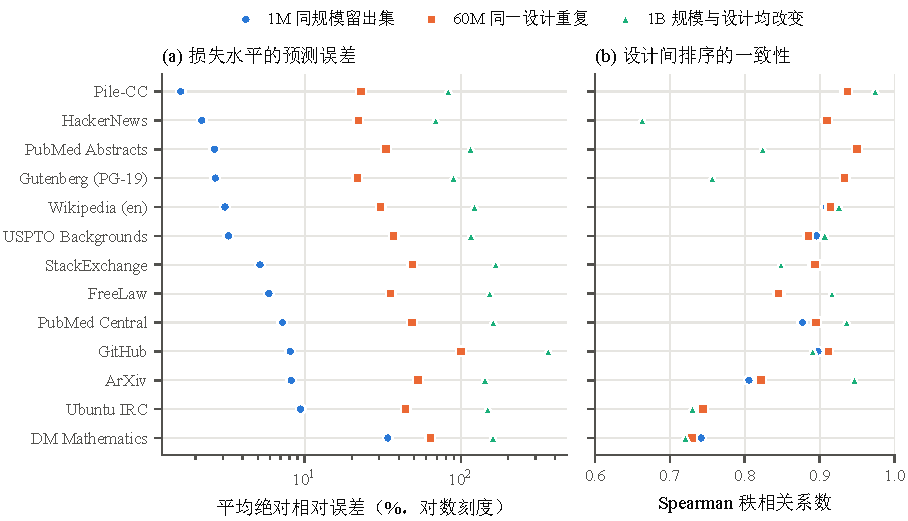
\includegraphics[width=\textwidth]{paper-q1-transfer}
  \caption{配比模型在三类检验集上的逐目标表现：(a) 平均绝对相对误差（对数刻度）；
           (b) 预测值与观测值在设计之间的 Spearman 秩相关}
  \label{fig:q1-transfer}
\end{figure}

\textbf{领域效应。}在 A4 配比中心把 0.01 的份额由 Pile-CC 转给某一领域，该领域自身的验证
损失在全部 12 个可计算的情形中都下降，降幅为 0.0305（Wikipedia）至 0.1686（DM Mathematics）；
196 个跨领域效应中有 85 个的条件区间不含 0，存在替代与互补并存的结构。这些效应以冻结的模型
形式和惩罚参数为条件，只描述 1M 规模的响应面，不是领域质量的因果效应。

\subsection{质量评分与配比的结合}

A16 给出的参考映射只能把 17 个配比领域中的 6 个关联到质量领域，其余 11 个没有质量信息，
本文不为其插补任何评分。定义配比的已映射质量占比 $m(\boldsymbol{p})=\sum_{d\in\mathcal{M}}p_d$
与已映射部分的条件平均质量
\begin{equation}
  Q(\boldsymbol{p})=\frac{\sum_{d\in\mathcal{M}}p_d\,Q_d}{m(\boldsymbol{p})},\qquad m(\boldsymbol{p})>0,
\end{equation}
$m(\boldsymbol{p})=0$ 时 $Q(\boldsymbol{p})$ 无定义。在 A4 的 512 个设计上，$m$ 的平均值为
0.5646，这是已映射领域在配比中的实际份额，而不是已映射领域个数与 17 之比。在 1M 响应面上，$Q(\boldsymbol{p})$
平均只解释各目标 6.8\% 的变化，且只有 3 个目标的斜率为负。因此质量评分不是配比的充分概括，
本文不把 $Q$ 作为配比模型的输入，两者作为互补的信息分别报告。

\subsection{外推稳健性}

A13 与 A15 是估算参照，不是 10B 与 70B 规模上的观测。把 1M 模型直接用于这两张表时，
13 个目标的平均相对误差分别为 202\% 与 286\%，只能作为压力诊断。结合 60M 与 1B 的检验结果，本文
不给出 10B/70B 的配比外推结论；能够跨规模保留的只有同一设计下配比排序的稳定性，而不是
损失的绝对水平。

\section{问题二的模型建立与求解}

\subsection{求解思路}

先在 B1 上估计经典标度律，并在任何结论之前检验 B1 的损失列是否含有真实训练噪声；再用独立
的观测表做外部验证；随后在半合成表上拟合包含质量的候选形式，按预先设定的采纳条件决定
是否把它作为广义标度律；最后在候选形式下推导边际效用、弹性与质量–规模替代条件。

\subsection{经典标度律的估计}

以 $N$（参数个数）与 $D$（Token 数）的原始计数拟合式 \eqref{eq:classic}。沿用
Hoffmann 等\cite{hoffmann2022chinchilla}的做法，对 $\log L$ 的残差取 Huber 损失\cite{huber1964robust}
（$\delta=10^{-3}$），并以 L-BFGS-B 算法\cite{byrd1995lbfgsb}从 108 个初值出发求全局最优。不采用对数线性最小二乘，因为它隐含 $E=0$，会把不可约损失
吸收进指数。

B1 由同一模型族的 8 条训练轨迹组成，对应 Pythia 系列的 8 个规模\cite{biderman2023pythia}，
共 1176 个检查点。同一轨迹上的检查点高度相关，因此不确定性以轨迹为重抽样单位
（假设 4）。表\ref{tab:q2-params}并列报告三类诊断：以轨迹为单位的自助法区间、逐一删去
一条轨迹后的参数范围，以及剖面目标函数——把某一参数固定为估计值的
$1\pm2\%$ 并重新优化其余参数后，目标函数相对最小值的倍数。

\begin{table}[htbp]
  \centering
  \caption{经典标度律参数及三类不确定性诊断}
  \label{tab:q2-params}
  \begin{tabular}{ccccc}
    \toprule
    参数 & 估计值 & 自助法 95\% 区间 & 删一轨迹范围 & 剖面倍数（$-2\%$/$+2\%$） \\
    \midrule
    $E$ & 1.68982 & [1.6897, 1.6899] & [1.68982, 1.68984] & 346.7 / 385.4 \\
    $A$ & 406.268 & [405.477, 406.776] & [406.154, 406.636] & 2.953 / 2.855 \\
    $\alpha$ & 0.339983 & [0.339867, 0.340051] & [0.339966, 0.340033] & 65.66 / 65.03 \\
    $B$ & 409.744 & [409.393, 410.090] & [409.615, 409.891] & 5.024 / 4.795 \\
    $\beta$ & 0.279888 & [0.279846, 0.279930] & [0.279871, 0.279906] & 80.14 / 78.67 \\
    \bottomrule
  \end{tabular}
\end{table}

三类诊断回答不同的问题，不能互相替代。删一轨迹的范围在全部 5 个参数上都窄于自助法区间：
自助法有放回地抽取 8 条轨迹，单次重抽样可能重复或遗漏多条轨迹，扰动远强于只删去一条；
任何单条轨迹对参数的影响都不超过其估计值的 0.0905\%。剖面倍数在偏离 2\% 时均明显大于 1，
说明 5 个参数都被数据确定。

\subsection{主拟合数据的生成公式识别}

上述区间极窄，这正是需要先解释的现象。把 Hoffmann 等\cite{hoffmann2022chinchilla}发表的常数
（$E=1.69$，$A=406.4$，$\alpha=0.34$，$B=410.7$，$\beta=0.28$）不经拟合直接代入 B1，
其中位绝对相对误差为 $3.24\times10^{-5}$，而 B1 以 4 位小数存储所对应的舍入量级为
$2.11\times10^{-5}$，二者之比仅 1.54，没有为真实训练噪声留下余地。作为对照，同样的检验在
半合成表 B2 上相差 21413 倍，说明该检验能区分不同性质的数据，而非对任何表都给出同一结论。

因此 B1 的损失列与“按已发表公式逐点计算”一致。在 B1 上拟合经典标度律，证明的是估计方法
能够恢复生成公式——重新拟合得到的参数与发表值的差异不超过 0.24\%——而\textbf{不是}对真实
模型规模规律的新发现，表\ref{tab:q2-params}中的窄区间也不代表对真实规律的精确认识。
关于真实模型的经验证据只能来自下面的独立验证。

\subsection{外部验证与有效域}
\label{sec:q2-validity}

\begin{table}[htbp]
  \centering
  \caption{经典标度律的外部验证}
  \label{tab:q2-validation}
  \begin{tabular}{lcccl}
    \toprule
    数据 & 性质 & 行数 & 中位绝对相对误差 & 说明 \\
    \midrule
    B5 文献数据 & 观测 & 44 & 7.52\% & 独立的模型族与机构 \\
    B4 剔除同族行 & 观测 & 49 & 8.07\% & 剔除后才构成盲验证 \\
    B4 含同族行 & 观测 & 57 & 8.62\% & 含信息泄漏，仅作对照 \\
    B2 & 半合成 & 1029 & 32.15\% & 校准数据，非观测证据 \\
    \bottomrule
  \end{tabular}
\end{table}

在独立的观测数据上，经典标度律的中位相对误差约为 8\%（表\ref{tab:q2-validation}）。
模型的有效域为 B1 覆盖的范围：$N\in[7.054\times10^{7},\,1.197\times10^{10}]$，
$D\in[1.340\times10^{8},\,2.999\times10^{11}]$；在此之外的计算均属外推。赛题要求结合
B9、B10 讨论百亿参数以上的外推：B9 只给出大模型的规格而无损失列，B10 是组织方提供的模型
输出，以 B10 拟合再以 B10 检验会构成循环论证，二者都不能检验外推的正确性。因此本文对
有效域以外、包括百亿参数以上的预测一律按外推表述，并注明其距有效域的距离。

\subsection{包含数据质量的候选形式及其采纳检验}

以“质量改变数据的有效规模”为出发点，考虑候选形式
\begin{equation}
  L(N,D,Q)=E+A N^{-\alpha}+B\left(Q^{\gamma}D\right)^{-\beta},\qquad \gamma>0,
  \label{eq:candidate}
\end{equation}
当 $Q=1$ 时它退化为经典形式。Subramanyam 等\cite{subramanyam2026quality}从有效样本量的角度
提出的质量感知标度律中，数据项为 $B/(D^{\beta}Q^{\gamma'})$，与式 \eqref{eq:candidate} 在
$\gamma'=\gamma\beta$ 时相同，二者属于同一函数族。可同时观测 $N,D,Q$ 与损失的只有半合成表：B6 的 360 行
完全包含于 B7 的 450 行（共享格点上损失完全一致），故只用 B7；B8 的质量方向与 B7 在全部
150 个审计格点上相反，其语义在现有材料中无法确定，予以隔离，不参与任何拟合。

在 B7 上拟合式 \eqref{eq:candidate} 得 $\hat\gamma=1.189$，$\hat\beta=0.0699$，
二者之积 $\hat\gamma\hat\beta=0.0831$。逐一留出一个质量水平的检验中，候选形式的
$\log L$ 预测误差比不含质量的基线降低 37.6\%。这些数值只说明候选形式在半合成表内部的
近似能力，属于半合成校准结果，不是关于真实模型的观测结论。

采纳条件在拟合前固定，包括参数取值、方向稳定、内部有效、可识别性、与真实 1M 数据的一致性
和与经典规律的兼容性，且要求候选的质量轴与问题一的质量评分之间存在第一方映射。结果为：
\begin{enumerate}
  \item \textbf{可识别性不通过。}在 $\gamma$ 的剖面上，把 $\gamma$ 改为估计值的 0.9 倍或
        1.1 倍，目标函数只增大 0.8\% 与 0.5\%；$\gamma$ 变化 4 倍时乘积 $\gamma\beta$ 只
        变化 1.29 倍，数据约束的是乘积而不是 $\gamma$ 本身；
  \item \textbf{与真实 1M 数据的一致性不通过。}问题一的配比质量 $Q(\boldsymbol{p})$ 与
        1M 宏平均损失的 Spearman 相关为 $-0.025$，按已映射份额分为三档后分别为 0.056、
        0.024、$-0.093$，没有稳定的“质量越高损失越低”关系；
  \item \textbf{与经典规律的兼容性不通过。}候选形式的 $N$--$D$ 部分在剔除同族行的 B4 上
        中位误差为 9.88\%，超过经典规律的 8.07\%；且质量项只在 $D\ge10^{10}$ 的范围内被识别；
  \item \textbf{不存在第一方映射。}B7 的质量取值是半合成设计变量，而问题一的 $Q$ 是以 A1
        为参照的相对秩评分，二者单调相关或取值范围相近都不能证明尺度等价。
\end{enumerate}
因此本文\textbf{不采纳}包含质量的广义标度律。可用于后续问题的标度律是经典形式
\eqref{eq:classic}，其中不含质量维度；问题一的质量评分与 1M 配比响应面作为独立的
信息保留，不与标度律合成为跨规模的质量规律。配比 $\boldsymbol{p}$ 同样不进入标度律：
$Q(\boldsymbol{p})$ 不是配比的充分概括，而配比响应面只在 1M 上有效。

\subsection{边际效用、弹性与质量–规模替代条件}

以下结论是式 \eqref{eq:candidate} 的解析推论，对任意正参数成立，不依赖任何数值估计；
它们回答“若质量以该形式进入标度律，会有什么结构”，而不构成经验结论。

\textbf{边际效用。}
\begin{equation}
  \frac{\partial L}{\partial N}=-\alpha A N^{-\alpha-1}<0,\quad
  \frac{\partial L}{\partial D}=-\beta B Q^{-\gamma\beta}D^{-\beta-1}<0,\quad
  \frac{\partial L}{\partial Q}=-\gamma\beta B Q^{-\gamma\beta-1}D^{-\beta}<0 .
\end{equation}

\textbf{弹性。}记 $\varepsilon_X=\partial\ln L/\partial\ln X$，则
\begin{equation}
  \varepsilon_N=-\frac{\alpha A N^{-\alpha}}{L},\qquad
  \varepsilon_D=-\frac{\beta B (Q^{\gamma}D)^{-\beta}}{L},\qquad
  \varepsilon_Q=\gamma\,\varepsilon_D .
\end{equation}
质量弹性恰为数据弹性的 $\gamma$ 倍：在该形式下，质量的作用完全通过数据项实现，数据项在
损失中占比越小，提升质量的收益越小。

\textbf{替代条件。}沿等损失曲线 $\mathrm{d}N/\mathrm{d}Q=-L_Q/L_N<0$，即提高质量可减少
达到同一损失所需的参数量。把质量由 $Q_0$ 提升到 $Q_1$ 使数据项下降
\begin{equation}
  R=B D^{-\beta}\left(Q_0^{-\gamma\beta}-Q_1^{-\gamma\beta}\right)>0 .
\end{equation}
若要在质量不变的情况下只靠增加参数获得同样的损失下降，所需参数量 $N'$ 满足
$A N'^{-\alpha}=A N^{-\alpha}-R$，即
\begin{equation}
  N'=\left(N^{-\alpha}-R/A\right)^{-1/\alpha},\qquad
  \Delta N=N'-N .
  \label{eq:equiv}
\end{equation}
式 \eqref{eq:equiv} 有限当且仅当 $R<A N^{-\alpha}$：质量提升带来的收益一旦超过参数项
剩余的全部可下降空间，就不存在与之等价的参数增量。“质量提升 0.1 等价于参数增加多少”
由此可在给定 $(N,D,Q_0)$ 下直接计算；但由于式 \eqref{eq:candidate} 未被采纳，本文不把
任何具体数值作为真实模型的结论。同样的原因使问题三无法在算力上比较“提升质量”与“扩大规模”
两条路径：在已采纳的经典形式中质量不降低损失，只消耗算力（第 \ref{sec:q3} 节）。

\section{问题三的模型建立与求解}
\label{sec:q3}

\subsection{求解思路}

问题三在问题二采纳的经典标度律 \eqref{eq:classic} 上求解算力约束下的资源配置。先按赛题给出的
三项开销建立算力成本模型；再在经典标度律的有效域内求解“损失最小、总算力不超过预算”的优化问题，
区分无可行解、预算用尽与预算有剩余三种情形；然后以最优解的约束激活状态定义“结构性转移”，在赛题
给出的预算范围内逐一识别；最后分析上下文长度、参数估计与质量成本函数对结论的影响。本节所有
数值都是已采纳标度律在有效域内的模型条件推论（B 类），描述模型给出的最优配置，而不是对真实
训练的观测或建议。

\subsection{算力成本模型}

按赛题给出的开销结构，训练、长文本注意力与质量提升三项开销分别为
\begin{equation}
  C_{\mathrm{train}}=6ND,\qquad
  C_{\mathrm{attn}}=\eta N D L_{\mathrm{ctx}},\qquad
  C_{Q}=D\left[g(Q)-g(Q_0)\right]_{+},
  \label{eq:q3-costs}
\end{equation}
其中 $\eta=2\times10^{-4}$，$[x]_{+}=\max\{x,0\}$，$g(Q)$ 是把单位 Token 的质量由基线 $Q_0$ 提升到
$Q$ 的成本函数（FLOPs/Token）。训练开销 $6ND$ 与 Hoffmann 等\cite{hoffmann2022chinchilla}求解
算力最优配置时采用的近似一致。总开销不得超过预算：
\begin{equation}
  C_{\mathrm{total}}=D\left[(6+\eta L_{\mathrm{ctx}})N+\left[g(Q)-g(Q_0)\right]_{+}\right]\le C .
  \label{eq:q3-budget}
\end{equation}
模型中的全部系数均与赛题原文逐项核对。记 $\kappa=6+\eta L_{\mathrm{ctx}}$，它是每个参数处理
每个 Token 所需的算力。在质量基线 $Q=Q_0$ 下 $[g(Q_0)-g(Q_0)]_{+}=0$，质量开销恰为零，约束化为
$\kappa ND\le C$。

在已花费的算力中，训练与注意力开销的占比分别为 $6/\kappa$ 与 $\eta L_{\mathrm{ctx}}/\kappa$，
只取决于上下文长度而与预算无关：$L_{\mathrm{ctx}}=4096$ 时为 88.0\% 与 12.0\%，
$L_{\mathrm{ctx}}=131072$ 时为 18.6\% 与 81.4\%。二者在 $L_{\mathrm{ctx}}=6/\eta=30000$ 时相等。
这只是一个成本恒等式：30000 不是最优上下文长度，不是区间转换点，也不是优化得到的临界值，
它本身也不是 C7 中出现的取值（观测值 8192 与 32768 位于其两侧）。

\subsection{优化模型与可行域}

经典标度律只在其拟合数据覆盖的范围内得到识别，本文把这一范围作为决策变量的可行域（有效域），
其边界为 $N_{\min}=7.054\times10^{7}$、$N_{\max}=1.197\times10^{10}$、$D_{\min}=1.340\times10^{8}$、
$D_{\max}=2.999\times10^{11}$（第 \ref{sec:q2-validity} 节）。在质量基线下，优化问题为
\begin{equation}
  \begin{aligned}
    \min_{N,D}\quad & L(N,D)=E+A N^{-\alpha}+B D^{-\beta}\\
    \text{s.t.}\quad & \kappa N D\le C,\qquad N_{\min}\le N\le N_{\max},\qquad D_{\min}\le D\le D_{\max}.
  \end{aligned}
  \label{eq:q3-problem}
\end{equation}
记 $C_{\min}=\kappa N_{\min}D_{\min}$ 与 $C_{\mathrm{box}}=\kappa N_{\max}D_{\max}$ 分别为有效域
下角点与上角点处的算力。由于 $L$ 对 $N$ 与 $D$ 都严格递减，问题 \eqref{eq:q3-problem} 的解分为
三种情形：
\begin{enumerate}
  \item $C<C_{\min}$：有效域内没有可行点；
  \item $C_{\min}\le C\le C_{\mathrm{box}}$：最优解使预算恰好用尽（$\kappa N^*D^*=C$），
        $C=C_{\mathrm{box}}$ 时它就是上角点；
  \item $C>C_{\mathrm{box}}$：有效域内的最优解是上角点 $(N_{\max},D_{\max})$，其余
        $C-C_{\mathrm{box}}$ 的预算未被使用。
\end{enumerate}
第三种情形是约束写成不等式的原因：若要求预算必须用尽，高预算下的解会被迫离开有效域，而在有效域
以外标度律没有得到识别。上角点只是有效域内的最优解，模型不给出有效域以外的最优配置，未使用的
预算也不意味着有用算力存在物理上限；本文不对未使用部分作任何外推或用途安排。

\subsection{求解方法与结构性转移的定义}

预算用尽时 $D=C/(\kappa N)$，问题化为关于 $N$ 的一维问题。其驻点为
\begin{equation}
  N_s=\left(\frac{\alpha A}{\beta B}\right)^{\frac{1}{\alpha+\beta}}
      \left(\frac{C}{\kappa}\right)^{\frac{\beta}{\alpha+\beta}},\qquad
  D_s=\frac{C}{\kappa N_s},
  \label{eq:q3-stationary}
\end{equation}
只有当驻点落在有效域内时它才是最优解；否则在有效域边界上求约束最优解，例如数据量取上界时
$D^*=D_{\max}$、$N^*=C/(\kappa D_{\max})$。求解结果与不使用任何解析候选的数值搜索一致，
$N^*$、$D^*$ 的相对差异不超过 $2.65\times10^{-10}$，并经有效域上的穷举网格检验。

\textbf{结构性转移的定义。}在给定上下文长度下，预算 $C$ 的\emph{区间}定义为：$C<C_{\min}$ 时为
“不可行”，否则为二元组（预算是否用尽，最优解处激活的全部有效域边界）。区间发生改变的预算称为
\textbf{结构性转移点}。在同一区间内最优解是预算的固定幂函数，因此转移点等价于预算弹性
$\mathrm{d}\ln N^*/\mathrm{d}\ln C$ 与 $\mathrm{d}\ln D^*/\mathrm{d}\ln C$ 的跳变点。
候选点为 $C_{\min}$、$C_{\mathrm{box}}$ 与驻点路径到达各边界时的预算；只有当约束最优解在候选点两侧
相对偏移 $\pm10^{-6}$ 处的区间确实不同时，候选点才被确认为转移点。分析范围限于赛题给出的预算
范围 $[10^{19},10^{24}]$ FLOPs，其中 $10^{19}$、$10^{22}$、$10^{24}$ 三个代表性预算为主要结果，
其间的连续预算用于识别转移点。

\subsection{配置结果}

表\ref{tab:q3-alloc}给出 $L_{\mathrm{ctx}}=4096$ 时三个代表性预算下的最优配置，图\ref{fig:q3-allocation}
给出五个上下文长度下最优配置随预算的变化。

\begin{table}[htbp]
  \centering
  \caption{代表性预算下的最优配置（$L_{\mathrm{ctx}}=4096$，$\kappa=6.8192$，质量基线）}
  \label{tab:q3-alloc}
  \setlength{\tabcolsep}{4.5pt}
  \begin{tabular}{ccccccc}
    \toprule
    预算 $C$ & $N^*$ & $D^*$ & 预测损失 & 区间 & 未用算力 & 利用率 \\
    \midrule
    $10^{19}$ & $2.152\times10^{8}$ & $6.814\times10^{9}$ & 3.0114 & 内点最优 & 0 & 1 \\
    $10^{22}$ & $4.890\times10^{9}$ & $2.999\times10^{11}$ & 2.1475 & 数据量取上界 & 0 & 1 \\
    $10^{24}$ & $1.197\times10^{10}$ & $2.999\times10^{11}$ & 2.0934 & 上角点，有剩余 & $9.755\times10^{23}$ & 0.0245 \\
    \bottomrule
    \multicolumn{7}{l}{\footnotesize 注：预算与算力单位为 FLOPs，$N^*$ 单位为个，$D^*$ 单位为 Token；三行的质量开销均为 0。}
  \end{tabular}
\end{table}

\begin{figure}[htbp]
  \centering
  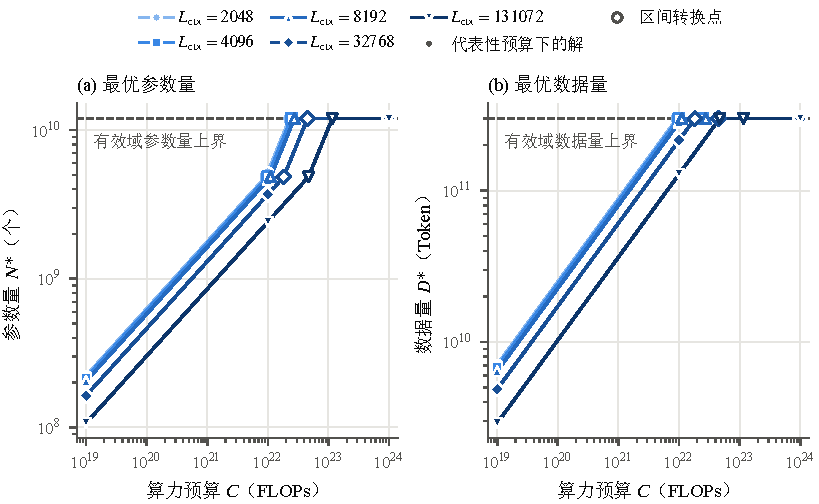
\includegraphics[width=\textwidth]{paper-q3-allocation}
  \caption{最优参数量与数据量随算力预算的变化（五个观测上下文长度；实心标记为代表性预算下的解，
           空心标记为区间转换点）}
  \label{fig:q3-allocation}
\end{figure}

\textbf{$10^{19}$ FLOPs：内点最优。}驻点落在有效域内，预算用尽，$N^*=2.152\times10^{8}$，
$D^*=6.814\times10^{9}$，预测损失 3.0114。此时 $N^*$ 与 $D^*$ 对预算的弹性分别为
$\beta/(\alpha+\beta)=0.4515$ 与 $\alpha/(\alpha+\beta)=0.5485$，即预算每增加 1\%，最优参数量约增加
0.45\%，最优数据量约增加 0.55\%。

\textbf{$10^{22}$ FLOPs：数据量达到有效域上界。}驻点所需的数据量已超过 $D_{\max}$，约束最优解取
$D^*=D_{\max}=2.999\times10^{11}$，$N^*=C/(\kappa D_{\max})=4.890\times10^{9}$，预算仍然用尽，
预测损失 2.1475。此区间内新增算力全部用于增加参数量（弹性为 1 与 0）。

\textbf{$10^{24}$ FLOPs：预算有剩余。}有效域上角点所需算力 $C_{\mathrm{box}}=2.447\times10^{22}$
远小于预算，最优解为上角点 $N^*=1.197\times10^{10}$、$D^*=2.999\times10^{11}$，预测损失 2.0934，
算力利用率为 0.0245，其余 $9.755\times10^{23}$ FLOPs 未被使用。赛题给出的最高预算已超过有效域
上角点所需的算力：在有效域内继续增加预算不再改变最优解，而有效域以外的配置不能由现有数据识别。

\textbf{结构性转移。}如图\ref{fig:q3-regimes}与表\ref{tab:q3-transitions}所示，在
$[10^{19},10^{24}]$ 内每个观测上下文长度都恰有两个转移点。第一个是驻点路径到达 $D_{\max}$ 的预算，
最优解由“内点最优”转为“数据量取上界”，预算弹性由 $(0.4515, 0.5485)$ 跳变为 $(1, 0)$；第二个是
$C_{\mathrm{box}}$，最优解到达上角点，此后预算出现剩余，弹性变为 $(0,0)$。前者是有效域边界
导致的约束激活变化，后者是有效域上界处开始出现预算剩余；$10^{19}$ 与 $10^{24}$ 只是分析范围的端点。
两类转移都是已采纳标度律有效域的性质，是模型内的陈述，本文不据此断言真实训练中存在物理意义上的
相变。$C_{\min}$（$6.06\times10^{16}$--$3.05\times10^{17}$）与驻点路径离开 $N_{\min}$ 的预算
（$7.95\times10^{17}$--$3.99\times10^{18}$）都低于 $10^{19}$，只作记录不作分析；范围内的每个
预算都有可行解。

\begin{figure}[htbp]
  \centering
  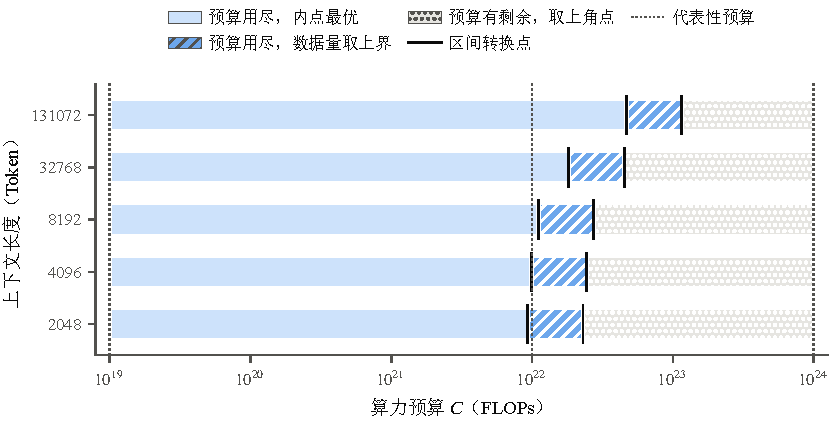
\includegraphics[width=\textwidth]{paper-q3-regimes}
  \caption{各观测上下文长度下最优解所处区间随预算的变化（上下文长度各占一行，行间不插值；
           竖实线为区间转换点，竖点线为三个代表性预算）}
  \label{fig:q3-regimes}
\end{figure}

\begin{table}[htbp]
  \centering
  \caption{各观测上下文长度下的结构性转移点（单位：FLOPs）}
  \label{tab:q3-transitions}
  \begin{tabular}{ccccc}
    \toprule
    \makecell{$L_{\mathrm{ctx}}$\\（Token）} & $\kappa$ & \makecell{内点最优 $\to$\\数据量取上界} &
    \makecell{数据量取上界 $\to$ 预算有剩余\\（即 $C_{\mathrm{box}}$）} & \makecell{$10^{24}$ FLOPs\\时的利用率} \\
    \midrule
    2048 & 6.4096 & $9.326\times10^{21}$ & $2.300\times10^{22}$ & 0.0230 \\
    4096 & 6.8192 & $9.922\times10^{21}$ & $2.447\times10^{22}$ & 0.0245 \\
    8192 & 7.6384 & $1.111\times10^{22}$ & $2.741\times10^{22}$ & 0.0274 \\
    32768 & 12.5536 & $1.827\times10^{22}$ & $4.505\times10^{22}$ & 0.0450 \\
    131072 & 32.2144 & $4.687\times10^{22}$ & $1.156\times10^{23}$ & 0.1156 \\
    \bottomrule
  \end{tabular}
\end{table}

\subsection{上下文长度的敏感性}

上下文长度只通过 $\kappa$ 进入模型：$L_{\mathrm{ctx}}$ 越大，每个参数处理每个 Token 的开销越高，
同一预算可支持的 $N D$ 越小。本文在 C7 中出现的 5 个上下文长度上逐一求解，不对上下文长度寻优，
也不在观测取值之间插值。在 $10^{19}$ FLOPs 下，$N^*$ 由 $2.213\times10^{8}$（2048）降至
$1.068\times10^{8}$（131072），$D^*$ 由 $7.050\times10^{9}$ 降至 $2.908\times10^{9}$，预测损失由
2.9989 升至 3.3672；两个转移点随上下文长度增大而移向更高的预算（表\ref{tab:q3-transitions}）。
因此在 $10^{22}$ FLOPs 下，上下文长度为 2048 与 4096 时数据量已取上界，而 8192 及以上时仍为内点
最优：观测值 4096 与 8192 夹住了这一区间变化，但现有网格不能确定变化发生在哪一个连续的上下文
长度上。在 $10^{24}$ FLOPs 下各上下文长度的最优解都是同一个上角点，算力利用率由 0.0230 升至
0.1156，差别只来自 $C_{\mathrm{box}}$ 随 $\kappa$ 增大。

\subsection{参数估计的稳健性}

问题二发布了 8 组“删去一条训练轨迹”后重新拟合的参数（6 位有效数字）。把每组参数代入同一有效域
与同一优化问题重新求解，得到最优配置的删一稳健性范围。$N^*$、$D^*$ 不受边界约束时，其相对范围为
$1.6\times10^{-4}$ 至 $3.8\times10^{-4}$，在发布精度下可以分辨；受边界约束时二者由边界确定，不随
参数变化。预测损失的相对范围为 $3.1\times10^{-6}$ 至 $1.8\times10^{-5}$，与把一组参数按 6 位有效数字
舍入所能造成的变化同量级，因此\textbf{在发布精度下无法分辨}，本文不就损失的差异下结论。第一个转移点
的相对范围为 $7.0\times10^{-4}$，没有一个范围包含代表性预算，名义拟合与 8 组删一拟合把每个代表性
预算都判入同一区间。

这些是删一稳健性范围，不是置信区间、自助法区间或后验区间。问题二只发布了各参数的边际自助法区间，
没有联合抽样，本文不从边际区间合成联合抽样，也不把剖面诊断转换为配置的界限。还需注意，问题二的
主拟合数据与已发表公式逐点一致，这些范围描述的是估计对删去单条轨迹的敏感性，不代表真实模型的
规模规律被确定到同样的精度。

\subsection{数据质量成本的处理}

赛题给出三族质量成本函数，$Q\in(0,1]$，单位为 FLOPs/Token：指数型 $\gamma e^{\lambda Q}$
（$\gamma=10^{7}$，$\lambda=6$）、幂函数型 $\gamma Q^{\lambda}$（$\gamma=5\times10^{9}$，$\lambda=4$）与
对数渐近型 $\gamma\ln(1+\lambda Q)$（$\gamma=2\times10^{9}$，$\lambda=10$）。围绕质量需要区分三个问题：
\begin{enumerate}
  \item \textbf{比较三族原始成本 $g(Q)$：可以完成。}这一比较不需要 $Q_0$，结果见下文与
        图\ref{fig:q3-quality}；
  \item \textbf{在配置中计入非基线的质量开销 $D[g(Q)-g(Q_0)]_{+}$：不能完成。}赛题只在语义上
        规定 $Q_0$ 取自附件 A 的质量评分或合理假设，没有给出全局数值；问题一的质量评分只覆盖
        17 个配比领域中的 6 个（已映射份额平均 0.5646），且是相对秩评分，本文既不把它当作 $Q_0$，
        也不为未映射的领域插补质量；
  \item \textbf{优化非平凡的质量水平：模型不支持。}已采纳的经典标度律不含质量项，把质量提高到
        $Q_0$ 以上只会占用本可用于 $N$ 与 $D$ 的算力，而不会降低模型预测的损失。这是模型形式的
        结果，不是“数据质量不重要”的判断；问题二中质量进入标度律的候选形式未能通过采纳检验，
        质量的收益因而无法以跨规模的方式计入。
\end{enumerate}

\begin{figure}[htbp]
  \centering
  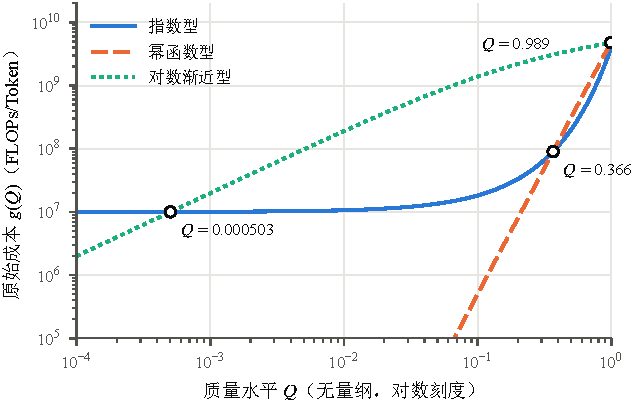
\includegraphics[width=0.74\textwidth]{paper-q3-quality-cost}
  \caption{三族质量成本函数的原始取值及其两两交点（双对数坐标，横轴只显示 $Q\in[10^{-4},1]$；
           为原始成本比较，不涉及 $Q_0$，也不是质量收益模型）}
  \label{fig:q3-quality}
\end{figure}

在 $(0,1]$ 上每两族恰好相交一次（图\ref{fig:q3-quality}）：指数型与对数渐近型交于
$Q=5.03\times10^{-4}$，指数型与幂函数型交于 $Q=0.366$，幂函数型与对数渐近型交于 $Q=0.989$。
交点个数由各对数差函数的单调分段解析确定，而非网格搜索。按原始成本由低到高，
$(0,5.03\times10^{-4})$ 上依次为幂函数型、对数渐近型、指数型；$(5.03\times10^{-4},0.366)$ 上为
幂函数型、指数型、对数渐近型；$(0.366,0.989)$ 上为指数型、幂函数型、对数渐近型；$(0.989,1]$ 上
为指数型、对数渐近型、幂函数型。没有一族在整个定义域上成本最低。原始成本的排序不等于配置所需的
增量成本 $g(Q)-g(Q_0)$ 的排序，后者取决于每一族在 $Q_0$ 与 $Q$ 之间的增量，在 $Q_0$ 确定之前
无法比较。

\subsection{结果的适用范围}

问题三的全部结论都以问题二采纳的经典标度律为前提，而该标度律在主拟合数据上只证明了生成公式
可以恢复；转移点描述的是标度律得到识别的范围，而不是训练在范围以外的行为。上下文长度的结论只
限于 5 个观测取值，区间变化只能被夹住而不能被定位；质量只在基线水平上计入，非基线的质量配置
须待 $Q_0$ 的数值确定后才能计算。

\section{问题四的模型建立与求解}

\subsection{求解思路}

先按预先固定的规则冻结分析总体与时间口径，再建立损失–得分映射并评估其能否支撑预测；
随后把历史得分变化分解为与规模相关和与规模无关的部分，并区分以参数量为尺度与以训练
算力为尺度的两种分解；最后以前沿得分的历史趋势给出延续基线，并在给定转移假设下分析
算力增长放缓的情景。本问所有时间趋势都是条件时间关联，不作因果解释。

\subsection{分析总体与口径}

\textbf{综合能力度量。}C1 的六项评测（IFEval、BBH、MATH Lvl 5、GPQA、MUSR、MMLU-PRO）
均已换算到相对随机基线的 0--100 尺度，且方向经核验均为越高越好；综合得分 $S$ 取六项
等权平均，即 C1 的 Average 字段（二者之差的最大绝对值为 $1.42\times10^{-14}$）。等权平均是透明的
概括而非按结果优化的权重，各单项结果同时保留。MATH Lvl 5 只使用 C1 汇总分。

\textbf{开源筛选。}模型须有公开权重的正向证据才入选：Hub 许可证属于宽松许可集合、Epoch
元数据标注开放权重，或权重可无限制访问，三者居其一。许可证属于宽松许可集合时视为允许研究
与复现；另两类信号只证明权重可以获取。缺乏任何信号的模型记为“未知”并排除，不记为闭源。

\textbf{模型类型。}预训练与持续预训练基础模型（A 组，215 个）与对话、指令微调及领域微调
模型（BC 组，1,170 个）始终分开分析，不合并为一条技术前沿。模型合并（D 类）没有独立的
训练过程，从主总体中排除，只在敏感性分析中重新纳入。

\textbf{时间口径。}有 Epoch 发布日期的模型取发布日期，否则取排行榜提交日期，每个模型保留
日期来源：主总体中 318 个为发布日期、1,067 个为提交日期。提交日期集中于 2024 年 6 月 8 日
至 2025 年 3 月 13 日，密集的历史只有 9 个月；若发布日期晚于该模型自身的提交日期 30 天以上，
则判定该发布日期不是该模型的发布日期，据此剔除 5 个模型。

按上述七条规则依次筛选后，4,497 个模型中保留 1,385 个。预测锚点取主总体最后的观测日期
2025 年 3 月 13 日，12 个月主预测与 24 个月压力预测分别对应 2026 年 3 月 13 日与 2027 年
3 月 13 日。

\subsection{损失–得分映射及其误差}

C5 的 43 个锚点完全包含于 C6 的 75 个锚点（取值一致），75 个锚点均按模型路径精确匹配到
排行榜记录。按组织方元数据在拟合前把锚点划分为三个可比性等级：S1 为与 B1 同族、同验证集的
7 个模型；S2 为 36 个跨族文献值，训练损失、验证损失与“最终”损失混杂；S3 为 32 个扩展变体，
其中 29 个的损失值来自另一个模型。S1 的 7 个损失与已发表标度律在其自身 $(N,D)$ 处的差异
不超过 $1.61\times10^{-4}$，与问题二的经典标度律处于同一损失尺度；但它们的综合得分为
5.07--6.06，全部处于评测下限附近。

在 S1 上预先声明常数、线性与 logit 线性三种非增映射，逐一留出锚点的 RMSE 分别为 0.424、
0.553 与 0.536，按一倍标准误准则选择常数映射：在损失区间 $[2.0933,\,2.5978]$ 内得分为
$5.66\pm0.42$。这意味着\textbf{在经典标度律的损失尺度上识别不出损失到得分的斜率}。
Schaeffer 等\cite{schaeffer2023mirage}指出，以非线性或不连续方式计分的下游指标，即使在逐 Token
损失平滑下降时也可能长期停留在下限附近；S1 锚点全部处于得分下限，与这一机制相容，但本文不据此
推断更低损失处的得分。S2 在同一模型族内能给出得分排序（族内 Spearman 相关为 $-1.000$ 至
$-0.232$），但跨族不能迁移：留出一个机构时，线性映射的 RMSE 为 10.31，反而高于常数映射的
9.64，因此各等级不合并。Ruan 等\cite{ruan2024observational}在公开模型的评测数据上同样注意到，
不同模型族的训练算力效率差异很大。

映射误差对结论的影响是决定性的：可比锚点全部位于得分下限，常数映射的误差就是全部预测
区间，任何经由损失换算得分的前沿预测都不可信。本文因此不给出基于损失–得分映射的前沿预测，
以下预测直接基于历史得分。Krajewski 等\cite{krajewski2026downstream}也不经由损失这一代理指标，
而是直接建立训练算力与下游准确率之间的关系；本文缺少覆盖前沿模型的训练算力数据，因而以时间
为自变量直接对历史得分建模。

\subsection{规模与非规模贡献的分解}

\textbf{参数规模分解。}对综合得分做回归 $S=a+b\log_{10}N+g\,t$，并记
$\log_{10}N=c+s\,t$。由遗漏变量恒等式，只对时间回归的斜率恰好等于 $g+b\,s$，其中
$b\,s$ 为与参数规模相关的部分，$g$ 为与规模无关的部分。后者包含一切在参数量固定时随时间
变化的因素，也包括训练数据量与算力的增长，本文称为“非规模相关的历史趋势”，不称为技术
进步或算法进步。

\begin{table}[htbp]
  \centering
  \caption{得分变化的分解（单位：分/年，括号内为 90\% 月块自助法区间）}
  \label{tab:q4-decomp}
  \begin{tabular}{lccc}
    \toprule
     & BC 组平均 & A 组平均 & A 组算力子集 \\
    规模尺度 & 参数量 & 参数量 & 训练算力 \\
    模型数 & 1,170 & 215 & 54 \\
    \midrule
    总趋势 & 5.32 [3.50, 7.18] & 1.36 [$-0.28$, 3.36] & 6.54 [4.58, 8.94] \\
    规模相关 & 0.58 [$-1.77$, 2.08] & $-1.03$ [$-3.16$, 0.74] & 4.30 [1.75, 6.78] \\
    非规模相关 & 4.74 [2.48, 8.06] & 2.39 [1.45, 3.82] & 2.24 [0.12, 4.51] \\
    规模占比 & 10.9\% [$-35$\%, 44\%] & 不报告$^{*}$ & 65.7\% [34\%, 98\%] \\
    \bottomrule
    \multicolumn{4}{l}{\footnotesize $^{*}$ 总趋势的区间包含 0，占比没有意义，只报告两个分量。} \\
  \end{tabular}
\end{table}

表\ref{tab:q4-decomp}显示，以参数量为尺度时，BC 组平均得分的年增幅中只有约十分之一与参数
规模相关，且区间跨过 0。以训练算力为尺度时结论不同：C4 只有 94 个模型能与面板关联，其中
62 个带有训练算力，占面板的 1.4\%，几乎全是预训练基础模型；在其中的 54 个 A 组模型上，与算力
相关的部分占 65.7\%。两种分解并不矛盾，训练算力同时随参数量与训练 Token 数增长，而参数量增长
不等于训练算力增长；算力分解只描述该子集，不推广到面板。按问题二的经典标度律做分解需要
$(N,D)$ 落在有效域内的模型，但满足条件的只有 6 个，且全部处于得分下限，该分解无法支撑结论。

\textbf{前沿分解。}前沿定义为综合得分的条件 90\% 分位数（对时间做线性分位数回归）。BC 组
在锚点处的前沿为 40.99（[39.57, 41.89]），前沿趋势为每年 9.91 分（[8.24, 12.53]），这一
直接时间趋势是预测的主要依据。预先声明的“按分位数的加性分解”未通过自身的一致性检验：分解
后的合计为 $-1.85$，而直接趋势为 9.91；按参数规模分段看，0--3B、3--10B、10--35B 与 35B
以上各段的前沿趋势分别为 0.35、5.42、8.60 与 24.92 分/年，差异很大。该分解作为负结果保留。
其后对前沿集合（每月得分不低于当月 90\% 分位数的 116 个模型）改用上述遗漏变量恒等式，
得到参数规模相关部分 $-0.59$（[$-6.12$, 1.92]）、非规模相关部分 11.38（[8.92, 17.45]）
分/年：前沿在上升的同时转向了更小的模型。该分解是在前述失败之后采用的，属于模型条件下的
事后分解，不是预先声明的方法，历史延续预测也不依赖它。

\subsection{前沿预测与不确定性}

问题要求在算力增长放缓的情景下预测前沿。本文给出三类数值，它们回答不同的问题，不能互相替代
（表\ref{tab:q4-forecast}）。

\begin{table}[htbp]
  \centering
  \caption{BC 组前沿预测（综合得分；括号内为区间）}
  \label{tab:q4-forecast}
  \begin{tabular}{>{\raggedright\arraybackslash}p{6.4cm}cc}
    \toprule
    预测类型 & 12 个月（主预测） & 24 个月（压力外推） \\
    \midrule
    历史延续基线 & 50.89 & 60.80 \\
    \quad 预测区间（90\%） & [45.72, 56.07] & [54.02, 67.57] \\
    \quad 含回测误差的预测区间 & [40.27, 61.52] & [49.31, 72.28] \\
    \quad 时间口径敏感性$^{*}$ & 50.89 / 50.37 / 65.31 & -- \\
    参数规模增长放缓（减半 / 停止） & 50.89 / 50.89 & 60.80 / 60.80 \\
    算力增长放缓的转移敏感性：减半 & 47.64 [46.06, 49.23] & 54.29 [51.12, 57.46] \\
    算力增长放缓的转移敏感性：停止 & 44.39 [41.22, 47.56] & 47.78 [41.44, 54.13] \\
    \bottomrule
    \multicolumn{3}{l}{\footnotesize $^{*}$ 依次为混合口径、仅用发布日期、仅用提交日期。} \\
  \end{tabular}
\end{table}

图\ref{fig:q4-frontier}(a) 给出 BC 组的月度前沿与延续基线，(b)(c) 把两个预测跨度上的各类数值
并列：菱形与细误差线是延续基线及其含回测误差的 90\% 预测区间；方块与粗线是把转移的算力占比
取其区间端点时预测值的变化范围，是敏感性范围而非概率区间；三角是只改变时间口径时的预测值。

\begin{figure}[htbp]
  \centering
  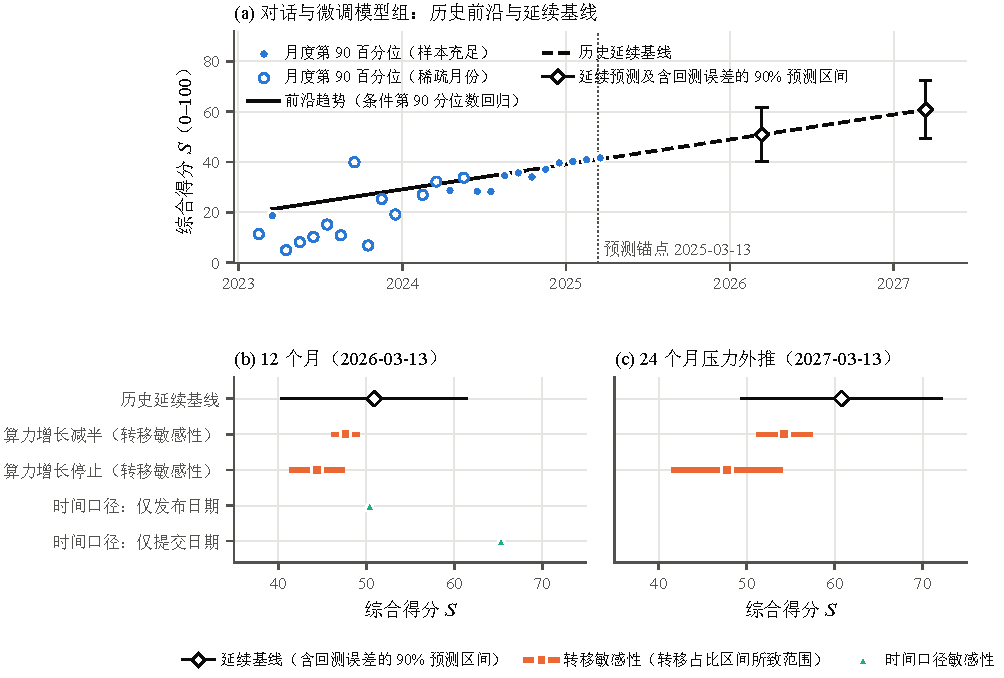
\includegraphics[width=\textwidth]{paper-q4-frontier}
  \caption{BC 组能力前沿的历史与预测：(a) 月度第 90 百分位（空心为模型数少于 20 的稀疏月份；
           2023 年以前的 3 个稀疏月份未画出）、前沿趋势与延续基线；(b)(c) 12 个月与 24 个月跨度上的
           延续基线、算力放缓的转移敏感性与时间口径敏感性}
  \label{fig:q4-frontier}
\end{figure}

\textbf{历史延续基线。}把前沿的直接时间趋势从锚点延续，12 个月为 50.89，24 个月为 60.80。
它回答的是“历史趋势延续会怎样”，并不是对算力放缓的经验回答。时间口径对它的影响大于模型
本身的不确定性：三种时间口径下的 12 个月预测为 50.37 至 65.31，跨度 14.94 分，超过模型
预测区间的宽度 10.34 分，仅用提交日期时的预测甚至落在该区间之外。本文不按预测结果挑选
时间口径，采用预先确定的混合口径并报告其敏感性。

\textbf{参数规模增长情景。}把与参数规模相关的前沿增长减半或停止，预测不变。原因是前沿的
参数规模相关部分不为正：前沿集合分解中规模相关部分占 $-5.5\%$，作用于直接趋势 9.91 分/年
即为 $-0.55$ 分/年，放缓它不会减少任何增长。这些是参数规模情景，
不是算力情景。

\textbf{算力增长放缓情景。}BC 组前沿没有具有代表性的历史算力数据，本文把 A 组算力子集上
估计的算力相关占比（65.7\%，区间 33.7\% 至 97.7\%）转移到 BC 组前沿趋势上，再对这一部分
减半或停止。所得 12 个月预测为 47.64（算力增长减半）与 44.39（停止），24 个月为 54.29 与
47.78，区间为转移占比取其区间端点时的范围。这是\textbf{在给定转移假设下的敏感性结果}，
不是已识别的总体效应，也不是因果效应。

\textbf{不确定性构成。}以 12 个月为例（标准差，单位为分），前沿水平与趋势外推两项分别为
0.81 与 1.39，整个前沿拟合的联合自助法标准差为 1.97；各月前沿点围绕拟合线的离散为 2.45；
二者按平方和合成的预测标准差为 3.14。24 个月时趋势外推一项增至 2.77，联合自助法为 3.31，
合成的预测标准差为 4.12。由于不使用损失–得分映射，
映射误差不进入这些区间。可验证的最长回测跨度为 6 个月（4 个起点），不声称 12 个月回测：
时间趋势模型的平均绝对误差为 5.49，偏差为 $-5.49$，每次回测都低估了前沿，故以含回测误差
的区间作为正式区间。

\textbf{其他敏感性。}纳入模型合并时 12 个月预测为 52.19，放宽开源条件时为 47.82，只用 B 组
或 C 组时分别为 55.07 与 50.17。A 组只有 3 个月份样本充足，无法回测，其 12 个月预测 34.30
（预测区间 [14.50, 54.09]）只作为未经验证的外推列出。

\subsection{逐任务分析与附件使用说明}

\textbf{逐任务聚合（C8）。}逐任务记录中通过汇总复现检验、并且具有真实子任务结构的是 BBH
（24 个子任务）与 MUSR（3 个子任务），共 1,860 个模型的 50,208 个子任务得分。以模型为组做
方差分解，模型间方差在 BBH 中只占 41.0\%、在 MUSR 中占 51.6\%，其余来自同一模型在不同
子任务上的差异：BBH 各子任务的中位得分从 0.00（跟踪乱序物体、谎言网络）到 60.00（布尔
表达式）不等，同一模型在 BBH 子任务间得分的标准差中位数为 19.52。汇总平均掩盖了这种不均衡，
因此综合得分只能描述整体水平，不能代表各项能力同步提升。MATH Lvl 5 的逐任务记录与汇总表
不一致（见第 4 节），未参与任何分析。

\textbf{辅助数据与元数据。}C3 作为辅助时间序列使用并经过核查：其“年份”是提交年份而非发布
年份，79 个模型有多条互不相同的得分，26 条历史记录不在排行榜第二版的得分尺度上，因此不作为
前沿观测。C4 提供训练算力、数据规模与开放权重信息，但只覆盖 94 个关联模型、其中 62 个带有
算力，且集中于预训练基础模型，所有基于 C4 的结论都只针对这一子集。

\section{模型分析检验}

\subsection{主要结论的证据等级}

不同检验支撑的结论强度不同。表\ref{tab:evidence}按第 \ref{sec:evidence-classes} 节的五个等级归类
各问的主要结论，同一问中的直接证据、模型条件推论、半合成校准、外推与敏感性分别表述，不互相替代。

\begin{table}[htbp]
  \centering
  \caption{各问主要结论的证据等级}
  \label{tab:evidence}
  \small
  \setlength{\tabcolsep}{4pt}
  \begin{tabular}{c>{\raggedright\arraybackslash}p{2.72cm}>{\raggedright\arraybackslash}p{2.72cm}%
                  >{\raggedright\arraybackslash}p{2.35cm}>{\raggedright\arraybackslash}p{2.95cm}%
                  >{\raggedright\arraybackslash}p{2.55cm}}
    \toprule
    问题 & A. 直接证据 & B. 模型条件推论 & C. 半合成校准 & D. 外推与敏感性 & E. 诊断与未决 \\
    \midrule
    问题一 & 域级质量评分与冲突率；1M 留出集检验通过 & 1M 响应面上的领域效应 & --- & 11 种方法变体；60M 与 1B 上的迁移检验；A13/A15 压力诊断 & 冲突成因未逐对检验 \\
    \addlinespace
    问题二 & B5、B4 盲验证的中位绝对相对误差 7.52\%、8.07\% & 候选形式下的边际效用、弹性与替代条件 & B7 上的候选形式（未采纳）；B2 对照 & 有效域以外的计算 & B1 的生成公式识别；B8 隔离 \\
    \addlinespace
    问题三 & --- & 各预算、各上下文长度下的最优配置与结构性转移点 & --- & 上下文长度敏感性；删一稳健性；三族原始质量成本比较 & 非基线质量配置待 $Q_0$ 确定 \\
    \addlinespace
    问题四 & 历史前沿与得分分解；算力子集（54 个模型）上的分解；6 个月回测 & 前沿集合的事后分解 & --- & 12/24 个月预测；算力放缓的转移敏感性；时间口径与总体定义 & 损失–得分映射识别不出斜率 \\
    \bottomrule
    \multicolumn{6}{l}{\footnotesize 注：“---”表示该问题在相应证据等级下无对应结论。} \\
  \end{tabular}
\end{table}

\subsection{灵敏度分析}

\textbf{问题一：}11 种预先声明的方法变体下，域级质量评分的最高与最低领域不变，中间领域的
排序随方法变化；缺失记录的三种极端取值使评分变化不超过 0.0002。配比模型的领域效应在 60M 的
配对设计上与 1M 保持 96.2\% 的符号一致，但在规模与设计同时改变的 1B 上只有 68.3\%。

\textbf{问题二：}删去任一条训练轨迹，参数变化不超过估计值的 0.0905\%；剖面目标函数在各参数
偏离 2\% 时都显著上升。二者说明参数由 B1 唯一确定，但由于 B1 与已发表公式逐点一致，这种
稳定性来自数据的生成方式，而不说明真实模型的规律同样确定。

\textbf{问题三：}上下文长度由 2048 增至 131072 时，两个转移点都移向更高的预算，$10^{19}$ FLOPs
下的最优参数量约减半；区间变化在观测取值之间只能被夹住。8 组删一参数下，不受边界约束的最优配置
相对变化不超过 $3.8\times10^{-4}$，每个代表性预算所处的区间不变；预测损失的差异在发布精度下
无法分辨。

\textbf{问题四：}12 个月预测对时间口径最敏感（50.37 至 65.31），其次是总体定义（纳入模型
合并、放宽开源条件、分组）与算力占比的转移区间；时间口径的影响超过模型本身的预测区间宽度。

\subsection{误差分析}

\textbf{问题一：}在同规模留出集上，13 个目标中 Pile-CC 的平均绝对相对误差最小（1.6\%，$R^2=0.865$），
DM Mathematics 最大（34.0\%，$R^2=0.413$），各领域的可预测程度差异明显，宏平均指标会掩盖
这种差异，逐目标结果见图\ref{fig:q1-transfer}。

\textbf{问题二：}按 B1 重新拟合的经典标度律在独立观测数据上的中位绝对相对误差约为 8\%；
它在拟合数据 B1 本身上的样本内中位绝对相对误差为 $3.26\times10^{-5}$，不是验证统计量，也不同于
第 \ref{sec:q2-generator} 节把已发表常数直接代入 B1 得到的 $3.24\times10^{-5}$。前者约 8\% 才是其对真实
模型的预测误差量级。

\textbf{问题三：}最优配置的数值误差来自求解与参数两方面：与不使用解析候选的数值搜索相比，
最优配置的相对差异不超过 $2.65\times10^{-10}$；参数方面的影响见上文的删一稳健性。这两项都不包含
经典标度律本身相对真实模型的误差（独立观测数据上的中位绝对相对误差约 8\%，第 \ref{sec:q2-validity} 节），
因此不能把配置结果的数值精度理解为对真实训练的预测精度。

\textbf{问题四：}6 个月回测中时间趋势模型的平均偏差为 $-5.49$ 分，每次都低估了前沿，说明
线性延续在近期是保守的；正式预测区间因此计入了回测误差。

\section{模型评价与推广}

\subsection{各问结论的衔接}

四个问题的结论沿同一条证据链衔接。问题一给出可复现的相对质量评分与 1M 规模上的配比响应面，
但响应面的损失水平不能跨规模迁移，质量评分也只覆盖 17 个配比领域中的 6 个；问题二因此只能采纳
不含质量的经典标度律，包含质量的候选形式作为未通过预设检验的结果保留，经典标度律在独立观测
数据上的中位相对误差约为 8\%；问题三在这一标度律的有效域内求解，最优配置随预算依次经过内点最优、
数据量取上界、预算有剩余三个区间，最高代表性预算中只有很小一部分能在有效域内使用，质量只能以
基线计入；问题四在经典标度律的损失尺度上识别不出损失到得分的斜率，因此不经由标度律换算，而直接
以历史得分给出 12 个月的前沿延续基线 50.89，并把算力增长放缓表述为给定转移假设下的敏感性结果。
前一问没有识别的关系，后一问都没有当作已知条件使用；各问的否定性结论与肯定性结论一样，界定了
本文结论的适用范围。

\subsection{模型的优点}

\begin{enumerate}
  \item \textbf{证据分级贯穿全文。}直接证据、模型条件推论、半合成校准、外推与敏感性、诊断与
        未决始终分开表述；在拟合前检验主数据的性质，避免把生成公式的恢复误认为新规律的发现。
  \item \textbf{判据预先设定。}配比模型的选择规则、广义标度律的采纳条件、分析总体与时间口径
        都在查看结果之前固定，否定性结论（广义形式不采纳、跨规模不迁移、映射无斜率）同样作为
        结果报告。
  \item \textbf{约束与转移有明确的数学定义。}算力约束保留为不等式并限定在有效域内求解，区分预算
        用尽与预算有剩余；结构性转移定义为约束激活状态的改变，并以预算弹性的跳变检验。
  \item \textbf{不确定性按数据结构度量。}质量评分按文档自助、标度律按训练轨迹重抽样、
        前沿按整月块自助，并把时间口径、总体定义等方法选择的影响单独列出。
\end{enumerate}

\subsection{模型的不足}

\begin{enumerate}
  \item 质量评分是相对代理量，冲突成因的解释来自领域分布模式，未对具体指标对逐一检验。
  \item 配比响应面只在 1M 规模上可作绝对预测，现有数据不足以支持向 10B/70B 的外推。
  \item 质量未能以可检验的方式进入标度律；经典标度律的经验支持只来自两张较小的独立观测表。
  \item 资源配置以经典标度律为前提，而该标度律在主拟合数据上只证明了生成公式可以恢复；上下文
        长度只有 5 个观测取值；质量基线 $Q_0$ 没有数值，非基线的质量配置未能计算。
  \item 前沿预测依赖 9 个月的密集历史和线性趋势假设，时间口径的影响大于模型本身的不确定性；
        算力放缓情景依赖从预训练子集转移而来的占比。
\end{enumerate}

\subsection{模型的推广}

体系平衡的质量聚合与冲突度量适用于任何多打分器的数据筛选场景；在拟合前用已发表公式检验
数据是否由公式生成的做法，可推广到一切使用组织方或第三方汇编数据的建模任务；有效域内的不等式
约束配置与以约束激活状态定义的结构性转移，适用于其他只在有限范围内得到识别的资源配置模型，一旦
给定 $Q_0$ 的数值和质量进入损失的可检验形式，非基线的质量配置也可以在同一框架中计算；把以参数量与
以训练算力为尺度的分解并列，可用于评估其他领域中规模扩张的贡献。


\bibliographystyle{gmcm}
\bibliography{references}

\appendix
% The appendix restarts the section counter, so its hyperlink anchors must be
% named apart from the body's, or its bookmarks resolve to section 1.
\renewcommand{\theHsection}{appendix.\Alph{section}}
\renewcommand{\theHsubsection}{appendix.\Alph{section}.\arabic{subsection}}
\renewcommand{\theHtable}{appendix.\Alph{section}.\arabic{table}}
\renewcommand{\theHfigure}{appendix.\Alph{section}.\arabic{figure}}
\renewcommand{\theHequation}{appendix.\Alph{section}.\arabic{equation}}
\section{复现与补充说明}
% Appendix-local numbering. The class restarts the section counter at
% \appendix, but ctex prints \thesection there as the full "附录 A" label, so
% subsections, tables, figures and equations are numbered A.1, A.2 explicitly.
\renewcommand{\thesubsection}{\Alph{section}.\arabic{subsection}}
\renewcommand{\thetable}{\Alph{section}.\arabic{table}}
\renewcommand{\thefigure}{\Alph{section}.\arabic{figure}}
\renewcommand{\theequation}{\Alph{section}.\arabic{equation}}
\setcounter{table}{0}
\setcounter{figure}{0}
\setcounter{equation}{0}

\subsection{运行环境、随机数种子与路径约定}

全部结果由提交材料中的程序生成。运行环境由 \texttt{environment.yml} 定义：Python 3.11.16、
NumPy 2.4.6、SciPy 1.17.1、pandas 3.0.6、PyYAML 6.0.3，作图另用 matplotlib-base 3.11.2。
问题一、问题二的主拟合与问题四的自助法使用 \texttt{configs/default.yaml} 中的种子 42，问题二的
不确定性与稳健性分析使用种子 20260923；问题三的求解程序与作图程序不使用随机数。

所有路径都相对于仓库根目录。原始附件只读，位于
\texttt{data\_local/\allowbreak problem-f/\allowbreak raw/}；生成的表格写入
\texttt{results/\allowbreak tables/}，图写入 \texttt{results/\allowbreak figures/}。

\subsection{复现入口}

各问的入口程序见表\ref{tab:repro}，均以如下命令运行：
\begin{center}
  \texttt{conda run -n modeling-research-2026 python} \textit{入口程序}
\end{center}
四个复现入口都会完整运行两遍、
逐字节比较生成结果，并核对原始输入在运行前后未被改动；问题三与问题四的入口还要求运行环境与
\texttt{environment.yml} 中固定的版本一致。面板构建程序生成的各表由问题四的复现入口核对不变。
作图程序在绘图前逐项核对所画数值与结果表一致，并附有植入错误的自检程序。

\begin{table}[htbp]
  \centering
  \caption{复现入口}
  \label{tab:repro}
  \begin{tabular}{ll}
    \toprule
    内容 & 入口程序 \\
    \midrule
    问题一：质量评价、冲突与配比 & \texttt{scripts/q1\_reproduce.py} \\
    问题二：标度律与广义形式检验 & \texttt{scripts/q2\_reproduce.py} \\
    问题三：配置与结构性转移 & \texttt{scripts/q3\_reproduce.py} \\
    问题四：排行榜面板 & \texttt{scripts/q4\_panel\_build.py} \\
    问题四：分解与前沿预测 & \texttt{scripts/q4\_evolution\_reproduce.py} \\
    正文图 & \texttt{scripts/paper\_figures.py} \\
    正文图的自检 & \texttt{scripts/paper\_figures\_selftest.py} \\
    \bottomrule
  \end{tabular}
\end{table}

\subsection{正文图表与结果文件的对应}

正文中的数值均取自 \texttt{results/tables/} 下的结果文件，主要对应关系见表\ref{tab:artifacts}。
五幅图的输入与输出的 SHA-256 记录在 \texttt{results/tables/paper-figures.md} 中。

\begin{table}[htbp]
  \centering
  \caption{正文图表与结果文件的对应}
  \label{tab:artifacts}
  \begin{tabular}{>{\raggedright\arraybackslash}p{3.2cm}>{\raggedright\arraybackslash}p{12.2cm}}
    \toprule
    正文图表 & 结果文件（\texttt{results/tables/} 下） \\
    \midrule
    表\ref{tab:q1-domain} & \texttt{q1-quality-analysis.md}，\texttt{q1-a1-a3-comparison.md} \\
    表\ref{tab:q1-validation}，图\ref{fig:q1-transfer} & \texttt{q1-mixture-validation.md} \\
    表\ref{tab:q2-params} & \texttt{q2-classic-fit.md}，\texttt{q2-uncertainty-robustness.md} \\
    表\ref{tab:q2-validation} & \texttt{q2-classic-fit.md} \\
    表\ref{tab:q3-alloc}，表\ref{tab:q3-transitions} & \texttt{q3-allocation.md}，\texttt{q3-context-sensitivity.md}，\texttt{q3-regime-thresholds.md} \\
    图\ref{fig:q3-allocation}，图\ref{fig:q3-regimes} & \texttt{q3-context-sensitivity.json}，\texttt{q3-regime-thresholds.json} \\
    图\ref{fig:q3-quality} & \texttt{q3-quality-cost-sensitivity.json} \\
    表\ref{tab:q4-decomp} & \texttt{q4-decomposition.md} \\
    表\ref{tab:q4-forecast}，图\ref{fig:q4-frontier} & \texttt{q4-frontier-forecast.md}，\texttt{q4-forecast-robustness.md} \\
    \bottomrule
  \end{tabular}
\end{table}


\end{document}
